% TODO: change the PATH
%\pdfminorversion=4 % for acroread
%\documentclass[aspectratio=169,t,xcolor={usenames,dvipsnames}]{beamer}
\documentclass[aspectratio=169,t,handout,xcolor={usenames,dvipsnames}]{beamer}
\usepackage{../beamerstyle}
\usepackage{dsfont}
\usepackage{bm}
\usepackage[english]{babel}
\usepackage[utf8]{inputenc}
\usepackage{graphicx}
\usepackage{algorithm}
\usepackage[ruled,vlined,algo2e,linesnumbered]{algorithm2e}
%\usepackage[boxed,vlined]{algorithm2e}
\usepackage{hyperref}
\usepackage{booktabs}
\usepackage{mathtools}

\usepackage{amsmath,amssymb}
\usepackage{listings}
\lstset{frame=lines,framesep=3pt,numbers=left,numberblanklines=false,basicstyle=\ttfamily\small}

\usepackage{subfig}
\usepackage{multicol}
%\usepackage{appendixnumberbeamer}
%
\usepackage{tcolorbox}

\usepackage{pgfplots}
\usepackage{tikz}
\usetikzlibrary{trees} 
\usetikzlibrary{shapes.geometric}
\usetikzlibrary{positioning,shapes,shadows,arrows,calc,mindmap}
\usetikzlibrary{positioning,fadings,through}
\usetikzlibrary{decorations.pathreplacing}
\usetikzlibrary{intersections}
\usetikzlibrary{positioning,fit,calc,shadows,backgrounds}
\pgfdeclarelayer{background}
\pgfdeclarelayer{foreground}
\pgfsetlayers{background,main,foreground}
\tikzstyle{activity}=[rectangle, draw=black, rounded corners, text centered, text width=8em]
\tikzstyle{data}=[rectangle, draw=black, text centered, text width=8em]
\tikzstyle{myarrow}=[->, thick, draw=black]

% Define the layers to draw the diagram
\pgfdeclarelayer{background}
\pgfdeclarelayer{foreground}
\pgfsetlayers{background,main,foreground}

%\usepackage{listings}
%\lstset{numbers=left,
%  showstringspaces=false,
%  frame={tb},
%  captionpos=b,
%  lineskip=0pt,
%  basicstyle=\ttfamily,
%%  extendedchars=true,
%  stepnumber=1,
%  numberstyle=\small,
%  xleftmargin=1em,
%  breaklines
%}

 
\definecolor{blue}{RGB}{0, 74, 153}

\usetheme{Boadilla}
%\useinnertheme{rectangles}
\usecolortheme{whale}
\setbeamercolor{alerted text}{fg=blue}
\useoutertheme{infolines}
\setbeamertemplate{navigation symbols}{\vspace{-5pt}} % to lower the logo
\setbeamercolor{date in head/foot}{bg=white} % blue
\setbeamercolor{date in head/foot}{fg=white}
\setbeamercolor{author  in head/foot}{bg=white} %blue
\setbeamercolor{title in head/foot}{bg=white} % blue
\setbeamercolor{title}{fg=white, bg=blue}
\setbeamercolor{block title}{fg=white,bg=blue}
\setbeamercolor{block body}{bg=blue!10}
\setbeamercolor{frametitle}{fg=white, bg=blue}
\setbeamercovered{invisible}

\makeatletter
\setbeamertemplate{footline}
{
  \leavevmode%
  \hbox{%
  \begin{beamercolorbox}[wd=.333333\paperwidth,ht=2.25ex,dp=1ex,center]{author in head/foot}%
%    \usebeamerfont{author in head/foot}\insertshortauthor
  \end{beamercolorbox}%
  \begin{beamercolorbox}[wd=.333333\paperwidth,ht=2.25ex,dp=1ex,center]{title in head/foot}%
    \usebeamerfont{title in head/foot}\insertshorttitle
  \end{beamercolorbox}%
  \begin{beamercolorbox}[wd=.333333\paperwidth,ht=2.25ex,dp=1ex,right]{date in head/foot}%
    \usebeamerfont{date in head/foot}\insertshortdate{}\hspace*{2em}
%    \insertframenumber\hspace*{2ex} 
  \end{beamercolorbox}}%
  \vskip0pt%
}
\makeatother

%\pgfdeclareimage[height=1.2cm]{automl}{images/logos/automl.png}
%\pgfdeclareimage[height=1.2cm]{freiburg}{images/logos/freiburg}

%\logo{\pgfuseimage{freiburg}}

\renewcommand{\comment}[1]{
	\noindent
	%\vspace{0.25cm}
	{\color{red}{\textbf{TODO:} #1}}
	%\vspace{0.25cm}
}
\newcommand{\notefh}[1]{\textcolor{red}{\textbf{FH:} #1}}
\renewcommand{\comment}[1]{}
\newcommand{\hide}[1]{}
\newcommand{\cemph}[2]{\emph{\textcolor{#1}{#2}}}

\newcommand{\lit}[1]{{\footnotesize\color{black!60}[#1]}}

\newcommand{\litw}[1]{{\footnotesize\color{blue!20}[#1]}}


\newcommand{\myframe}[2]{\begin{frame}[c]{#1}#2\end{frame}}
\newcommand{\myframetop}[2]{\begin{frame}{#1}#2\end{frame}}
\newcommand{\myit}[1]{\begin{itemize}#1\end{itemize}}
\newcommand{\myblock}[2]{\begin{block}{#1}#2\end{block}}


\newcommand{\votepurple}[1]{\textcolor{Purple}{$\bigstar$}}
\newcommand{\voteyellow}[1]{\textcolor{Goldenrod}{$\bigstar$}}
\newcommand{\voteblue}[1]{\textcolor{RoyalBlue}{$\bigstar$}}
\newcommand{\votepink}[1]{\textcolor{Pink}{$\bigstar$}}

\newcommand{\diff}{\mathop{}\!\mathrm{d}}
\newcommand{\refstyle}[1]{{\small{\textcolor{gray}{#1}}}}
\newcommand{\hands}[0]{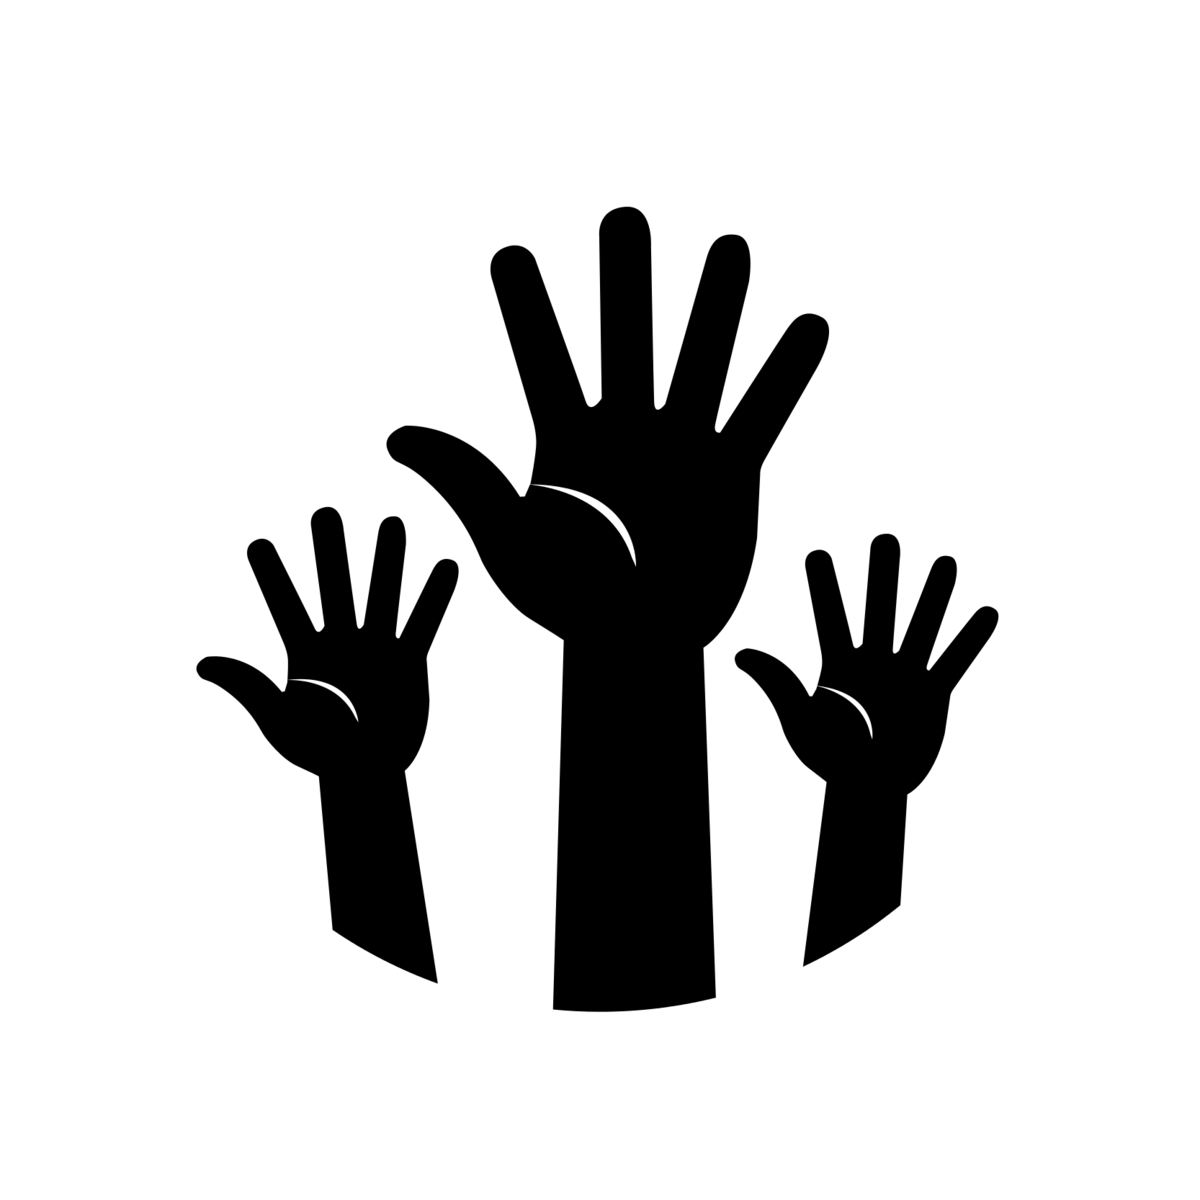
\includegraphics[height=1.5em]{images/hands}}
\newcommand{\transpose}[0]{{\textrm{\tiny{\sf{T}}}}}
\newcommand{\norm}{{\mathcal{N}}}
\newcommand{\cutoff}[0]{\kappa}
\newcommand{\instD}[0]{\dataset}
\newcommand{\insts}[0]{\mathcal{I}}
\newcommand{\inst}[0]{i}
\newcommand{\instI}[1]{i^{(#1)}}

% Iteration specific instance of variable/function/anything
% Introduced in the BO section, but moved up here to make it available within other macros
\newcommand{\iter}[2][\bocount]{{#2}^{(#1)}}

%--------HPO parameter macros-----------

% Parameter Configuration Space
\newcommand{\pcs}[0]{\pmb{\Lambda}}

% ???
\newcommand{\bx}[0]{\conf}

% Parameter Configuration
\newcommand{\conf}[0]{\pmb{\lambda}}

% Final Configuration
\newcommand{\finconf}[0]{\pmb{\hat{\lambda}}}

% Configuration corresponding to a given iteration -- better use \iter!
\newcommand{\confI}[1]{{\conf}^{(#1)}}

% Default Configuration
\newcommand{\defconf}[0]{{\conf}_{\text{def}}}

% Incumbent Configuration
\newcommand{\incumbent}[1][\bocount]{\iter[#1]{\finconf}}

% Optimal Configuration
\newcommand{\optconf}[0]{{\conf}^*}

% Configuration Space
\newcommand{\confs}[0]{\pcs}

%----------------------------------------

%\newcommand{\vlambda}[0]{\bm{\lambda}}
%\newcommand{\vLambda}[0]{\bm{\Lambda}}
\newcommand{\dataset}[0]{\mathcal{D}}
\newcommand{\datasets}[0]{\mathbf{D}}
\newcommand{\loss}[0]{L}
\newcommand{\risk}{\mathcal{R}}
\newcommand{\riske}{\mathcal{R}_{\text{emp}}}
\newcommand{\cost}[0]{c}
\newcommand{\costI}[1]{c^{(#1)}}

% Gaussian Process
\newcommand{\gp}{\mathcal{G}}
% Family of Objective Functions
\newcommand{\objF}{F}

%---------------BO Macros------------------

% BO loop counter
\newcommand{\bocount}{t}
% BO loop counter max, the counter runs from 1 to this value
\newcommand{\bobudget}{T}
% BO loop observation
\newcommand{\obs}[1][\conf]{\cost({#1})}
% BO loop observation space
\newcommand{\obsspace}{\mathcal{Y}}
% BO loop next observation
\newcommand{\bonextobs}{\obs[\iter{\conf}]}
% Acquisition Function, no args
\newcommand{\acq}{u}
% Standard Normal PDF
\newcommand{\pdf}{\phi}
% Standard Normal CDF
\newcommand{\cdf}{\Phi}
% Mean
\newcommand{\mean}{\mu}
% Standard Deviation
\newcommand{\stddev}{\sigma}
% Variance
\newcommand{\variance}{\sigma^2}
% Noise
\newcommand{\noise}{\nu}
% BO loop next selected sample
\newcommand{\bonextsample}{\confI{\bocount}}

% Single hyperparameter
\newcommand{\hyperparam}{\lambda}

% Single hyperparameter within a hyperparameter configuration
\newcommand{\hyperparami}[1][i]{{\hyperparam}_#1}

% Full definition of final configuration
\newcommand{\finconffull}{\incumbent[\bobudget]}

% Dataset
\newcommand{\datasetHPO}{{\dataset}_{HPO}}

% Dataset definition
\newcommand{\datasetHPOdef}{{\langle \bonextsample,\,\bonextobs \rangle}_{\bocount=1}^{\bobudget}}

% Double Display Fraction, forces large displays for everything in numerator and denominator
\newcommand\ddfrac[2]{\frac{\displaystyle #1}{\displaystyle #2}}

% Conditional Probability "Given That" Relation, source:https://tex.stackexchange.com/a/141685/205886
\newcommand\given[1][]{\:#1\vert\:}

% Expectation as a math operator
\DeclareMathOperator*{\E}{\mathbb{E}}

% Citation 
\newcommand{\source}[1]{
    \begin{flushright}
    	Source: \lit{#1}
    \end{flushright}
}
%-------------------------------------------

%Real numbers set
\newcommand{\realnum}{\mathbb{R}}
%Configuration space - do not use
%\newcommand{\configspace}{\Theta}
%Instances - do not use
%\newcommand{\instances}{\mathcal{I}}
%Expected value
\newcommand{\expectation}{\mathbb{E}}
%Kernel
\newcommand{\kernel}{\kappa}
%Constraint function
\newcommand{\constraintf}{c}
%Normal distribution
\newcommand{\normaldist}{\mathcal{N}}

% \renewcommand{\vec}[1]{\mathbf{#1}}
\newcommand{\hist}[0]{\dataset_{\text{Hist}}}
\newcommand{\param}[0]{p}
\newcommand{\algo}[0]{\mathcal{A}}
\newcommand{\algos}[0]{\mathbf{A}}
%\newcommand{\nn}[0]{N}
\newcommand{\feats}[0]{\mathcal{X}_{\text{meta}}}
\newcommand{\feat}[0]{\x_{\text{meta}}}
%\newcommand{\cluster}[0]{\vec{h}}
%\newcommand{\clusters}[0]{\vec{H}}
\newcommand{\perf}[0]{\mathbb{R}}
%\newcommand{\surro}[0]{\mathcal{S}}
\newcommand{\surro}[0]{\hat{\cost}}
\newcommand{\func}[0]{f}
\newcommand{\epm}[0]{\surro}
\newcommand{\portfolio}[0]{\mathbf{P}}
\newcommand{\schedule}[0]{\mathcal{S}}

% Machine Learning
\newcommand{\mdata}[0]{\dataset_{\text{meta}}}
\newcommand{\datasettrain}[0]{\dataset_{\text{train}}}
\newcommand{\datasetval}[0]{\dataset_{\text{val}}}
\newcommand{\datasettest}[0]{\dataset_{\text{test}}}
\newcommand{\x}[0]{\mathbf{x}}
\newcommand{\y}[0]{y}
\newcommand{\xI}[1]{\mathbf{x}^{(#1)}}
\newcommand{\yI}[1]{y^{(#1)}}
\newcommand{\fx}{f(\mathbf{x})}  % f(x), continuous prediction function
\newcommand{\Hspace}{\mathcal{H}} % hypothesis space where f is from
\newcommand{\fh}{\hat{f}}       % f hat, estimated prediction function

% Deep Learning
\newcommand{\weights}[0]{\theta}
\newcommand{\metaweights}[0]{\phi}


% reinforcement learning
\newcommand{\policies}[0]{\mathbf{\Pi}}
\newcommand{\policy}[0]{\pi}
\newcommand{\actionRL}[0]{a}
\newcommand{\stateRL}[0]{s}
\newcommand{\statesRL}[0]{\mathcal{S}}
\newcommand{\rewardRL}[0]{r}
\newcommand{\rewardfuncRL}[0]{\mathcal{R}}

\RestyleAlgo{algoruled}
\DontPrintSemicolon
\LinesNumbered
\SetAlgoVlined
\SetFuncSty{textsc}

\SetKwInOut{Input}{Input}
\SetKwInOut{Output}{Output}
\SetKw{Return}{return}

%\newcommand{\changed}[1]{{\color{red}#1}}

%\newcommand{\citeN}[1]{\citeauthor{#1}~(\citeyear{#1})}

\renewcommand{\vec}[1]{\mathbf{#1}}
\DeclareMathOperator*{\argmin}{arg\,min}
\DeclareMathOperator*{\argmax}{arg\,max}

%\newcommand{\aqme}{\textit{AQME}}
%\newcommand{\aslib}{\textit{ASlib}}
%\newcommand{\llama}{\textit{LLAMA}}
%\newcommand{\satzilla}{\textit{SATzilla}}
%\newcommand{\satzillaY}[1]{\textit{SATzilla'{#1}}}
%\newcommand{\snnap}{\textit{SNNAP}}
%\newcommand{\claspfolioTwo}{\textit{claspfolio~2}}
%\newcommand{\flexfolio}{\textit{FlexFolio}}
%\newcommand{\claspfolioOne}{\textit{claspfolio~1}}
%\newcommand{\isac}{\textit{ISAC}}
%\newcommand{\eisac}{\textit{EISAC}}
%\newcommand{\sss}{\textit{3S}}
%\newcommand{\sunny}{\textit{Sunny}}
%\newcommand{\ssspar}{\textit{3Spar}}
%\newcommand{\cshc}{\textit{CSHC}}
%\newcommand{\cshcpar}{\textit{CSHCpar}}
%\newcommand{\measp}{\textit{ME-ASP}}
%\newcommand{\aspeed}{\textit{aspeed}}
%\newcommand{\autofolio}{\textit{AutoFolio}}
%\newcommand{\cedalion}{\textit{Cedalion}}
\newcommand{\fanova}{\textit{fANOVA}}
\newcommand{\sbs}{\textit{SB}}
\newcommand{\oracle}{\textit{VBS}}

% like approaches
\newcommand{\claspfoliolike}[1]{\texttt{claspfolio-#1-like}}
\newcommand{\satzillalike}[1]{\texttt{SATzilla'#1-like}}
\newcommand{\isaclike}{\texttt{ISAC-like}}
\newcommand{\ssslike}{\texttt{3S-like}}
\newcommand{\measplike}{\texttt{ME-ASP-like}}

\newcommand{\irace}{\textit{I/F-race}}
\newcommand{\gga}{\textit{GGA}}
\newcommand{\smac}{\textit{SMAC}}
\newcommand{\paramils}{\textit{ParamILS}}
\newcommand{\spearmint}{\textit{Spearmint}}
\newcommand{\tpe}{\textit{TPE}}


\usepackage{pifont}
\newcommand{\itarrow}{\mbox{\Pisymbol{pzd}{229}}}
\newcommand{\ithook}{\mbox{\Pisymbol{pzd}{52}}}
\newcommand{\itcross}{\mbox{\Pisymbol{pzd}{56}}}
\newcommand{\ithand}{\mbox{\raisebox{-1pt}{\Pisymbol{pzd}{43}}}}

%\DeclareMathOperator*{\argmax}{arg\,max}

\newcommand{\ie}{{\it{}i.e.\/}}
\newcommand{\eg}{{\it{}e.g.\/}}
\newcommand{\cf}{{\it{}cf.\/}}
\newcommand{\wrt}{\mbox{w.r.t.}}
\newcommand{\vs}{{\it{}vs\/}}
\newcommand{\vsp}{{\it{}vs\/}}
\newcommand{\etc}{{\copyedit{etc.}}}
\newcommand{\etal}{{\it{}et al.\/}}

\newcommand{\pscProc}{{\bf procedure}}
\newcommand{\pscBegin}{{\bf begin}}
\newcommand{\pscEnd}{{\bf end}}
\newcommand{\pscEndIf}{{\bf endif}}
\newcommand{\pscFor}{{\bf for}}
\newcommand{\pscEach}{{\bf each}}
\newcommand{\pscThen}{{\bf then}}
\newcommand{\pscElse}{{\bf else}}
\newcommand{\pscWhile}{{\bf while}}
\newcommand{\pscIf}{{\bf if}}
\newcommand{\pscRepeat}{{\bf repeat}}
\newcommand{\pscUntil}{{\bf until}}
\newcommand{\pscWithProb}{{\bf with probability}}
\newcommand{\pscOtherwise}{{\bf otherwise}}
\newcommand{\pscDo}{{\bf do}}
\newcommand{\pscTo}{{\bf to}}
\newcommand{\pscOr}{{\bf or}}
\newcommand{\pscAnd}{{\bf and}}
\newcommand{\pscNot}{{\bf not}}
\newcommand{\pscFalse}{{\bf false}}
\newcommand{\pscEachElOf}{{\bf each element of}}
\newcommand{\pscReturn}{{\bf return}}

%\newcommand{\param}[1]{{\sl{}#1}}
\newcommand{\var}[1]{{\it{}#1}}
\newcommand{\cond}[1]{{\sf{}#1}}
%\newcommand{\state}[1]{{\sf{}#1}}
%\newcommand{\func}[1]{{\sl{}#1}}
\newcommand{\set}[1]{{\Bbb #1}}
%\newcommand{\inst}[1]{{\tt{}#1}}
\newcommand{\myurl}[1]{{\small\sf #1}}

\newcommand{\Nats}{{\Bbb N}}
\newcommand{\Reals}{{\Bbb R}}
\newcommand{\extset}[2]{\{#1 \; | \; #2\}}

\newcommand{\vbar}{$\,\;|$\hspace*{-1em}\raisebox{-0.3mm}{$\,\;\;|$}}
\newcommand{\vendbar}{\raisebox{+0.4mm}{$\,\;|$}}
\newcommand{\vend}{$\,\:\lfloor$}


\newcommand{\goleft}[2][.7]{\parbox[t]{#1\linewidth}{\strut\raggedright #2\strut}}
\newcommand{\rightimage}[2][.3]{\mbox{}\hfill\raisebox{1em-\height}[0pt][0pt]{\includegraphics[width=#1\linewidth]{#2}}\vspace*{-\baselineskip}}




\pdfminorversion=4 % for acroread
%\documentclass[aspectratio=169,t,xcolor={usenames,dvipsnames}]{beamer}
\documentclass[aspectratio=169,t,handout,xcolor={usenames,dvipsnames}]{beamer}
\usepackage{../beamerstyle}
\usepackage{dsfont}
\usepackage{bm}
\usepackage[english]{babel}
\usepackage[utf8]{inputenc}
\usepackage{graphicx}
\usepackage{algorithm}
\usepackage[ruled,vlined,algo2e,linesnumbered]{algorithm2e}
%\usepackage[boxed,vlined]{algorithm2e}
\usepackage{hyperref}
\usepackage{booktabs}
\usepackage{mathtools}

\usepackage{amsmath,amssymb}
\usepackage{listings}
\lstset{frame=lines,framesep=3pt,numbers=left,numberblanklines=false,basicstyle=\ttfamily\small}

\usepackage{subfig}
\usepackage{multicol}
%\usepackage{appendixnumberbeamer}
%
\usepackage{tcolorbox}

\usepackage{pgfplots}
\usepackage{tikz}
\usetikzlibrary{trees} 
\usetikzlibrary{shapes.geometric}
\usetikzlibrary{positioning,shapes,shadows,arrows,calc,mindmap}
\usetikzlibrary{positioning,fadings,through}
\usetikzlibrary{decorations.pathreplacing}
\usetikzlibrary{intersections}
\usetikzlibrary{positioning,fit,calc,shadows,backgrounds}
\pgfdeclarelayer{background}
\pgfdeclarelayer{foreground}
\pgfsetlayers{background,main,foreground}
\tikzstyle{activity}=[rectangle, draw=black, rounded corners, text centered, text width=8em]
\tikzstyle{data}=[rectangle, draw=black, text centered, text width=8em]
\tikzstyle{myarrow}=[->, thick, draw=black]

% Define the layers to draw the diagram
\pgfdeclarelayer{background}
\pgfdeclarelayer{foreground}
\pgfsetlayers{background,main,foreground}

%\usepackage{listings}
%\lstset{numbers=left,
%  showstringspaces=false,
%  frame={tb},
%  captionpos=b,
%  lineskip=0pt,
%  basicstyle=\ttfamily,
%%  extendedchars=true,
%  stepnumber=1,
%  numberstyle=\small,
%  xleftmargin=1em,
%  breaklines
%}

 
\definecolor{blue}{RGB}{0, 74, 153}

\usetheme{Boadilla}
%\useinnertheme{rectangles}
\usecolortheme{whale}
\setbeamercolor{alerted text}{fg=blue}
\useoutertheme{infolines}
\setbeamertemplate{navigation symbols}{\vspace{-5pt}} % to lower the logo
\setbeamercolor{date in head/foot}{bg=white} % blue
\setbeamercolor{date in head/foot}{fg=white}
\setbeamercolor{author  in head/foot}{bg=white} %blue
\setbeamercolor{title in head/foot}{bg=white} % blue
\setbeamercolor{title}{fg=white, bg=blue}
\setbeamercolor{block title}{fg=white,bg=blue}
\setbeamercolor{block body}{bg=blue!10}
\setbeamercolor{frametitle}{fg=white, bg=blue}
\setbeamercovered{invisible}

\makeatletter
\setbeamertemplate{footline}
{
  \leavevmode%
  \hbox{%
  \begin{beamercolorbox}[wd=.333333\paperwidth,ht=2.25ex,dp=1ex,center]{author in head/foot}%
%    \usebeamerfont{author in head/foot}\insertshortauthor
  \end{beamercolorbox}%
  \begin{beamercolorbox}[wd=.333333\paperwidth,ht=2.25ex,dp=1ex,center]{title in head/foot}%
    \usebeamerfont{title in head/foot}\insertshorttitle
  \end{beamercolorbox}%
  \begin{beamercolorbox}[wd=.333333\paperwidth,ht=2.25ex,dp=1ex,right]{date in head/foot}%
    \usebeamerfont{date in head/foot}\insertshortdate{}\hspace*{2em}
%    \insertframenumber\hspace*{2ex} 
  \end{beamercolorbox}}%
  \vskip0pt%
}
\makeatother

%\pgfdeclareimage[height=1.2cm]{automl}{images/logos/automl.png}
%\pgfdeclareimage[height=1.2cm]{freiburg}{images/logos/freiburg}

%\logo{\pgfuseimage{freiburg}}

\renewcommand{\comment}[1]{
	\noindent
	%\vspace{0.25cm}
	{\color{red}{\textbf{TODO:} #1}}
	%\vspace{0.25cm}
}
\newcommand{\notefh}[1]{\textcolor{red}{\textbf{FH:} #1}}
\renewcommand{\comment}[1]{}
\newcommand{\hide}[1]{}
\newcommand{\cemph}[2]{\emph{\textcolor{#1}{#2}}}

\newcommand{\lit}[1]{{\footnotesize\color{black!60}[#1]}}

\newcommand{\litw}[1]{{\footnotesize\color{blue!20}[#1]}}


\newcommand{\myframe}[2]{\begin{frame}[c]{#1}#2\end{frame}}
\newcommand{\myframetop}[2]{\begin{frame}{#1}#2\end{frame}}
\newcommand{\myit}[1]{\begin{itemize}#1\end{itemize}}
\newcommand{\myblock}[2]{\begin{block}{#1}#2\end{block}}


\newcommand{\votepurple}[1]{\textcolor{Purple}{$\bigstar$}}
\newcommand{\voteyellow}[1]{\textcolor{Goldenrod}{$\bigstar$}}
\newcommand{\voteblue}[1]{\textcolor{RoyalBlue}{$\bigstar$}}
\newcommand{\votepink}[1]{\textcolor{Pink}{$\bigstar$}}

\newcommand{\diff}{\mathop{}\!\mathrm{d}}
\newcommand{\refstyle}[1]{{\small{\textcolor{gray}{#1}}}}
\newcommand{\hands}[0]{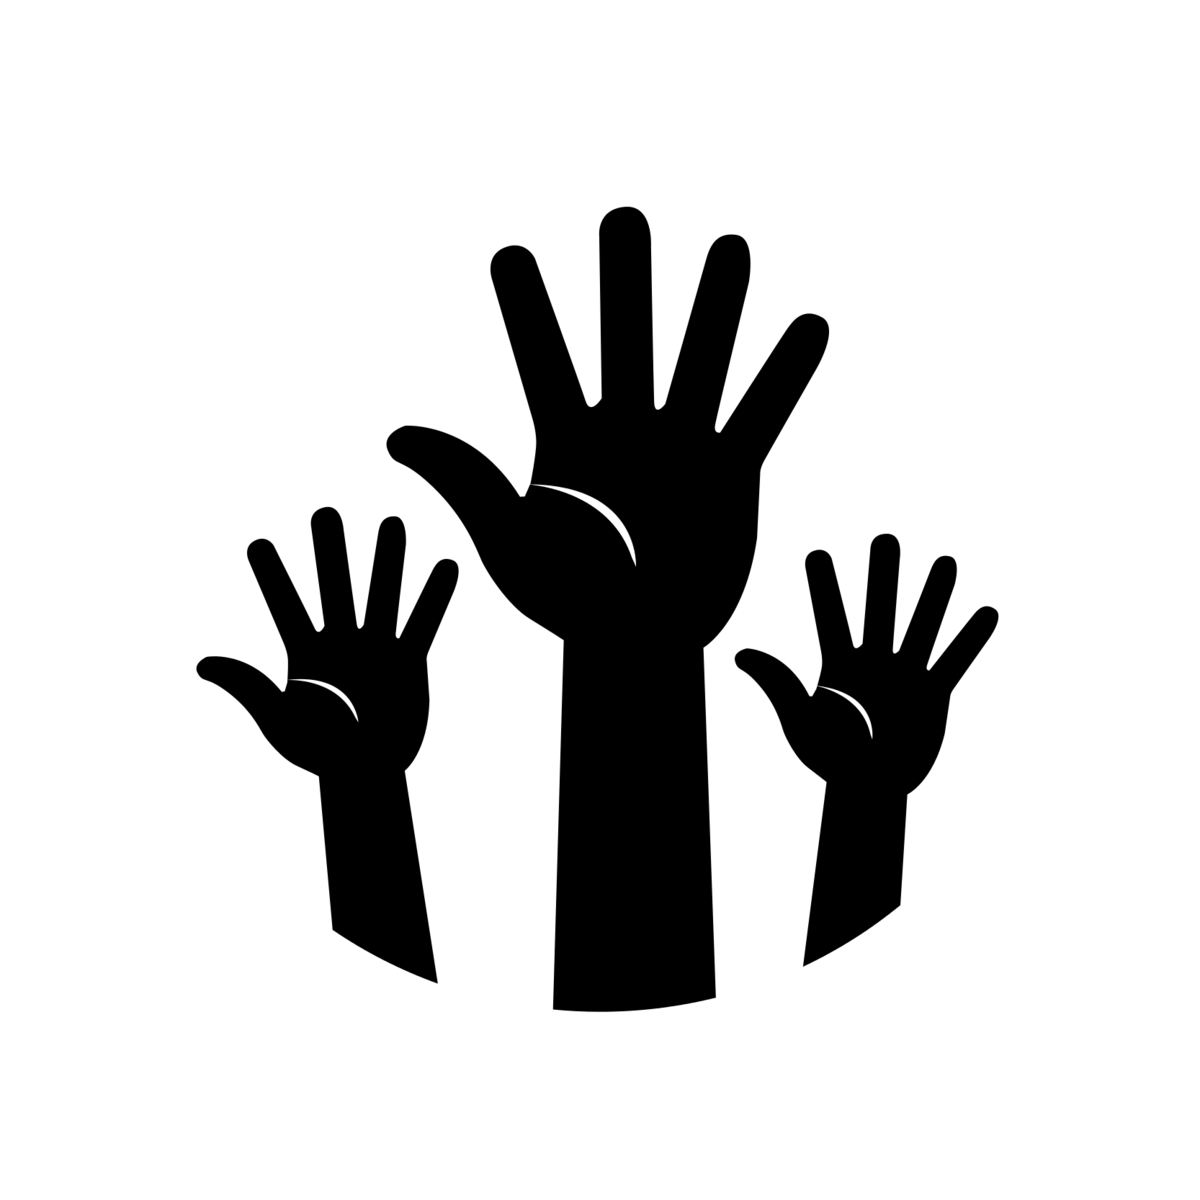
\includegraphics[height=1.5em]{images/hands}}
\newcommand{\transpose}[0]{{\textrm{\tiny{\sf{T}}}}}
\newcommand{\norm}{{\mathcal{N}}}
\newcommand{\cutoff}[0]{\kappa}
\newcommand{\instD}[0]{\dataset}
\newcommand{\insts}[0]{\mathcal{I}}
\newcommand{\inst}[0]{i}
\newcommand{\instI}[1]{i^{(#1)}}

% Iteration specific instance of variable/function/anything
% Introduced in the BO section, but moved up here to make it available within other macros
\newcommand{\iter}[2][\bocount]{{#2}^{(#1)}}

%--------HPO parameter macros-----------

% Parameter Configuration Space
\newcommand{\pcs}[0]{\pmb{\Lambda}}

% ???
\newcommand{\bx}[0]{\conf}

% Parameter Configuration
\newcommand{\conf}[0]{\pmb{\lambda}}

% Final Configuration
\newcommand{\finconf}[0]{\pmb{\hat{\lambda}}}

% Configuration corresponding to a given iteration -- better use \iter!
\newcommand{\confI}[1]{{\conf}^{(#1)}}

% Default Configuration
\newcommand{\defconf}[0]{{\conf}_{\text{def}}}

% Incumbent Configuration
\newcommand{\incumbent}[1][\bocount]{\iter[#1]{\finconf}}

% Optimal Configuration
\newcommand{\optconf}[0]{{\conf}^*}

% Configuration Space
\newcommand{\confs}[0]{\pcs}

%----------------------------------------

%\newcommand{\vlambda}[0]{\bm{\lambda}}
%\newcommand{\vLambda}[0]{\bm{\Lambda}}
\newcommand{\dataset}[0]{\mathcal{D}}
\newcommand{\datasets}[0]{\mathbf{D}}
\newcommand{\loss}[0]{L}
\newcommand{\risk}{\mathcal{R}}
\newcommand{\riske}{\mathcal{R}_{\text{emp}}}
\newcommand{\cost}[0]{c}
\newcommand{\costI}[1]{c^{(#1)}}

% Gaussian Process
\newcommand{\gp}{\mathcal{G}}
% Family of Objective Functions
\newcommand{\objF}{F}

%---------------BO Macros------------------

% BO loop counter
\newcommand{\bocount}{t}
% BO loop counter max, the counter runs from 1 to this value
\newcommand{\bobudget}{T}
% BO loop observation
\newcommand{\obs}[1][\conf]{\cost({#1})}
% BO loop observation space
\newcommand{\obsspace}{\mathcal{Y}}
% BO loop next observation
\newcommand{\bonextobs}{\obs[\iter{\conf}]}
% Acquisition Function, no args
\newcommand{\acq}{u}
% Standard Normal PDF
\newcommand{\pdf}{\phi}
% Standard Normal CDF
\newcommand{\cdf}{\Phi}
% Mean
\newcommand{\mean}{\mu}
% Standard Deviation
\newcommand{\stddev}{\sigma}
% Variance
\newcommand{\variance}{\sigma^2}
% Noise
\newcommand{\noise}{\nu}
% BO loop next selected sample
\newcommand{\bonextsample}{\confI{\bocount}}

% Single hyperparameter
\newcommand{\hyperparam}{\lambda}

% Single hyperparameter within a hyperparameter configuration
\newcommand{\hyperparami}[1][i]{{\hyperparam}_#1}

% Full definition of final configuration
\newcommand{\finconffull}{\incumbent[\bobudget]}

% Dataset
\newcommand{\datasetHPO}{{\dataset}_{HPO}}

% Dataset definition
\newcommand{\datasetHPOdef}{{\langle \bonextsample,\,\bonextobs \rangle}_{\bocount=1}^{\bobudget}}

% Double Display Fraction, forces large displays for everything in numerator and denominator
\newcommand\ddfrac[2]{\frac{\displaystyle #1}{\displaystyle #2}}

% Conditional Probability "Given That" Relation, source:https://tex.stackexchange.com/a/141685/205886
\newcommand\given[1][]{\:#1\vert\:}

% Expectation as a math operator
\DeclareMathOperator*{\E}{\mathbb{E}}

% Citation 
\newcommand{\source}[1]{
    \begin{flushright}
    	Source: \lit{#1}
    \end{flushright}
}
%-------------------------------------------

%Real numbers set
\newcommand{\realnum}{\mathbb{R}}
%Configuration space - do not use
%\newcommand{\configspace}{\Theta}
%Instances - do not use
%\newcommand{\instances}{\mathcal{I}}
%Expected value
\newcommand{\expectation}{\mathbb{E}}
%Kernel
\newcommand{\kernel}{\kappa}
%Constraint function
\newcommand{\constraintf}{c}
%Normal distribution
\newcommand{\normaldist}{\mathcal{N}}

% \renewcommand{\vec}[1]{\mathbf{#1}}
\newcommand{\hist}[0]{\dataset_{\text{Hist}}}
\newcommand{\param}[0]{p}
\newcommand{\algo}[0]{\mathcal{A}}
\newcommand{\algos}[0]{\mathbf{A}}
%\newcommand{\nn}[0]{N}
\newcommand{\feats}[0]{\mathcal{X}_{\text{meta}}}
\newcommand{\feat}[0]{\x_{\text{meta}}}
%\newcommand{\cluster}[0]{\vec{h}}
%\newcommand{\clusters}[0]{\vec{H}}
\newcommand{\perf}[0]{\mathbb{R}}
%\newcommand{\surro}[0]{\mathcal{S}}
\newcommand{\surro}[0]{\hat{\cost}}
\newcommand{\func}[0]{f}
\newcommand{\epm}[0]{\surro}
\newcommand{\portfolio}[0]{\mathbf{P}}
\newcommand{\schedule}[0]{\mathcal{S}}

% Machine Learning
\newcommand{\mdata}[0]{\dataset_{\text{meta}}}
\newcommand{\datasettrain}[0]{\dataset_{\text{train}}}
\newcommand{\datasetval}[0]{\dataset_{\text{val}}}
\newcommand{\datasettest}[0]{\dataset_{\text{test}}}
\newcommand{\x}[0]{\mathbf{x}}
\newcommand{\y}[0]{y}
\newcommand{\xI}[1]{\mathbf{x}^{(#1)}}
\newcommand{\yI}[1]{y^{(#1)}}
\newcommand{\fx}{f(\mathbf{x})}  % f(x), continuous prediction function
\newcommand{\Hspace}{\mathcal{H}} % hypothesis space where f is from
\newcommand{\fh}{\hat{f}}       % f hat, estimated prediction function

% Deep Learning
\newcommand{\weights}[0]{\theta}
\newcommand{\metaweights}[0]{\phi}


% reinforcement learning
\newcommand{\policies}[0]{\mathbf{\Pi}}
\newcommand{\policy}[0]{\pi}
\newcommand{\actionRL}[0]{a}
\newcommand{\stateRL}[0]{s}
\newcommand{\statesRL}[0]{\mathcal{S}}
\newcommand{\rewardRL}[0]{r}
\newcommand{\rewardfuncRL}[0]{\mathcal{R}}

\RestyleAlgo{algoruled}
\DontPrintSemicolon
\LinesNumbered
\SetAlgoVlined
\SetFuncSty{textsc}

\SetKwInOut{Input}{Input}
\SetKwInOut{Output}{Output}
\SetKw{Return}{return}

%\newcommand{\changed}[1]{{\color{red}#1}}

%\newcommand{\citeN}[1]{\citeauthor{#1}~(\citeyear{#1})}

\renewcommand{\vec}[1]{\mathbf{#1}}
\DeclareMathOperator*{\argmin}{arg\,min}
\DeclareMathOperator*{\argmax}{arg\,max}

%\newcommand{\aqme}{\textit{AQME}}
%\newcommand{\aslib}{\textit{ASlib}}
%\newcommand{\llama}{\textit{LLAMA}}
%\newcommand{\satzilla}{\textit{SATzilla}}
%\newcommand{\satzillaY}[1]{\textit{SATzilla'{#1}}}
%\newcommand{\snnap}{\textit{SNNAP}}
%\newcommand{\claspfolioTwo}{\textit{claspfolio~2}}
%\newcommand{\flexfolio}{\textit{FlexFolio}}
%\newcommand{\claspfolioOne}{\textit{claspfolio~1}}
%\newcommand{\isac}{\textit{ISAC}}
%\newcommand{\eisac}{\textit{EISAC}}
%\newcommand{\sss}{\textit{3S}}
%\newcommand{\sunny}{\textit{Sunny}}
%\newcommand{\ssspar}{\textit{3Spar}}
%\newcommand{\cshc}{\textit{CSHC}}
%\newcommand{\cshcpar}{\textit{CSHCpar}}
%\newcommand{\measp}{\textit{ME-ASP}}
%\newcommand{\aspeed}{\textit{aspeed}}
%\newcommand{\autofolio}{\textit{AutoFolio}}
%\newcommand{\cedalion}{\textit{Cedalion}}
\newcommand{\fanova}{\textit{fANOVA}}
\newcommand{\sbs}{\textit{SB}}
\newcommand{\oracle}{\textit{VBS}}

% like approaches
\newcommand{\claspfoliolike}[1]{\texttt{claspfolio-#1-like}}
\newcommand{\satzillalike}[1]{\texttt{SATzilla'#1-like}}
\newcommand{\isaclike}{\texttt{ISAC-like}}
\newcommand{\ssslike}{\texttt{3S-like}}
\newcommand{\measplike}{\texttt{ME-ASP-like}}

\newcommand{\irace}{\textit{I/F-race}}
\newcommand{\gga}{\textit{GGA}}
\newcommand{\smac}{\textit{SMAC}}
\newcommand{\paramils}{\textit{ParamILS}}
\newcommand{\spearmint}{\textit{Spearmint}}
\newcommand{\tpe}{\textit{TPE}}


\usepackage{pifont}
\newcommand{\itarrow}{\mbox{\Pisymbol{pzd}{229}}}
\newcommand{\ithook}{\mbox{\Pisymbol{pzd}{52}}}
\newcommand{\itcross}{\mbox{\Pisymbol{pzd}{56}}}
\newcommand{\ithand}{\mbox{\raisebox{-1pt}{\Pisymbol{pzd}{43}}}}

%\DeclareMathOperator*{\argmax}{arg\,max}

\newcommand{\ie}{{\it{}i.e.\/}}
\newcommand{\eg}{{\it{}e.g.\/}}
\newcommand{\cf}{{\it{}cf.\/}}
\newcommand{\wrt}{\mbox{w.r.t.}}
\newcommand{\vs}{{\it{}vs\/}}
\newcommand{\vsp}{{\it{}vs\/}}
\newcommand{\etc}{{\copyedit{etc.}}}
\newcommand{\etal}{{\it{}et al.\/}}

\newcommand{\pscProc}{{\bf procedure}}
\newcommand{\pscBegin}{{\bf begin}}
\newcommand{\pscEnd}{{\bf end}}
\newcommand{\pscEndIf}{{\bf endif}}
\newcommand{\pscFor}{{\bf for}}
\newcommand{\pscEach}{{\bf each}}
\newcommand{\pscThen}{{\bf then}}
\newcommand{\pscElse}{{\bf else}}
\newcommand{\pscWhile}{{\bf while}}
\newcommand{\pscIf}{{\bf if}}
\newcommand{\pscRepeat}{{\bf repeat}}
\newcommand{\pscUntil}{{\bf until}}
\newcommand{\pscWithProb}{{\bf with probability}}
\newcommand{\pscOtherwise}{{\bf otherwise}}
\newcommand{\pscDo}{{\bf do}}
\newcommand{\pscTo}{{\bf to}}
\newcommand{\pscOr}{{\bf or}}
\newcommand{\pscAnd}{{\bf and}}
\newcommand{\pscNot}{{\bf not}}
\newcommand{\pscFalse}{{\bf false}}
\newcommand{\pscEachElOf}{{\bf each element of}}
\newcommand{\pscReturn}{{\bf return}}

%\newcommand{\param}[1]{{\sl{}#1}}
\newcommand{\var}[1]{{\it{}#1}}
\newcommand{\cond}[1]{{\sf{}#1}}
%\newcommand{\state}[1]{{\sf{}#1}}
%\newcommand{\func}[1]{{\sl{}#1}}
\newcommand{\set}[1]{{\Bbb #1}}
%\newcommand{\inst}[1]{{\tt{}#1}}
\newcommand{\myurl}[1]{{\small\sf #1}}

\newcommand{\Nats}{{\Bbb N}}
\newcommand{\Reals}{{\Bbb R}}
\newcommand{\extset}[2]{\{#1 \; | \; #2\}}

\newcommand{\vbar}{$\,\;|$\hspace*{-1em}\raisebox{-0.3mm}{$\,\;\;|$}}
\newcommand{\vendbar}{\raisebox{+0.4mm}{$\,\;|$}}
\newcommand{\vend}{$\,\:\lfloor$}


\newcommand{\goleft}[2][.7]{\parbox[t]{#1\linewidth}{\strut\raggedright #2\strut}}
\newcommand{\rightimage}[2][.3]{\mbox{}\hfill\raisebox{1em-\height}[0pt][0pt]{\includegraphics[width=#1\linewidth]{#2}}\vspace*{-\baselineskip}}





% Bayesian Optimization SS 2020 macros
%%-----------------------------------
% Recommended format for this file:

%           *************
%           Section Title
%           *************


% % Macro n descriptive name
% \newcommand...
%
% % Macro n+1 full name
% \newcommand...
%------------------------------------

%           *************
%       Mathematical Notations
%           *************


% Note: The user should be responsible for enclosing these within $$ in order to simplify macro definition, e.g. when using \mathcal.


% Gaussian Process
\newcommand{\gp}{\mathcal{G}}

% Real Objective Function - do not use
%\newcommand{\objf}{f}

% Family of Objective Functions
\newcommand{\objF}{F}

% BO loop counter
\newcommand{\bocount}{t}

% BO loop counter max, the counter runs from 1 to this value
\newcommand{\bobudget}{T}

% BO parameter space
\newcommand{\boparamspace}{\mathcal{X}}

% BO parameter
\newcommand{\boparam}{x}

% BO current incumbent
\newcommand{\boincumb}{\boparam^+_\bocount}

% BO loop observation
\newcommand{\boobs}{y}

% BO loop observation space
\newcommand{\boobsspace}{\mathcal{Y}}

% BO loop next sample (selected for evaluation at each iteration of the BO loop)
\newcommand{\bonextsample}{\boparam_\bocount}

% BO loop next observation 
\newcommand{\bonextobs}{\boobs_\bocount}

% Surrogate Function, no args -- do not use
% \renewcommand{\surro}{\hat{f}}

% Acquisition Function, no args
\newcommand{\acq}{u}

% Dataset - do not use
%\renewcommand{\dataset}{\mathcal{D}}

% Standard Normal PDF
\newcommand{\pdf}{\phi}

% Standard Normal CDF
\newcommand{\cdf}{\Phi}

% Mean
\newcommand{\mean}{\mu}

% Standard Deviation
\newcommand{\stddev}{\sigma}

% Variance
\newcommand{\variance}{\sigma^2}

% Noise
\newcommand{\noise}{\nu}

%Real numbers set
\newcommand{\realnum}{\mathbb{R}}

%Configuration space - do not use
%\newcommand{\configspace}{\Theta}

%Instances
\newcommand{\instances}{\mathcal{I}}

%Expected value
\newcommand{\expectation}{\mathbb{E}}

%Kernel
\newcommand{\kernel}{\kappa}

%Constraint function
\newcommand{\constraintf}{c}

%Normal distribution
\newcommand{\normaldist}{\mathcal{N}}
%------------------------------------

%           *************
%         Convenience Macros
%           *************


% Double Display Fraction, forces large displays for everything in numerator and denominator
\newcommand\ddfrac[2]{\frac{\displaystyle #1}{\displaystyle #2}}

% Citation 
\newcommand{\source}[1]{
    \begin{flushright}
    	Source: \lit{#1}
    \end{flushright}
}

% Conditional Probability "Given That" Relation, source:https://tex.stackexchange.com/a/141685/205886
\newcommand\given[1][]{\:#1\vert\:}

% Expectation as a math operator
\DeclareMathOperator*{\E}{\mathbb{E}}

\title[AutoML: Grey-box Approaches]{Speedup Techniques for Hyperparameter Optimization}
\subtitle{Overview of the grey-box approaches}
%TODO: change authors!
\author[Frank Hutter]{Frank Hutter}
\institute{University of Freiburg}
\date{??.??.??}



\AtBeginSection[] % Do nothing for \section*
{
  \begin{frame}{Outline}
    \bigskip
    \vfill
    \tableofcontents[currentsection]
  \end{frame}
}

\begin{document}
	
	\maketitle
\section{Introduction to grey-box approaches}
%-------------------------------------------------
%-------------------------------------------------
\begin{frame}{Recall: Black-box optimization}
\begin{figure}
    \centering
    


\tikzset{every picture/.style={line width=0.75pt}} %set default line width to 0.75pt        

\begin{tikzpicture}[x=0.70pt,y=0.70pt,yscale=-1,xscale=1]
%uncomment if require: \path (0,300); %set diagram left start at 0, and has height of 300

%Straight Lines [id:da5075678478287002] 
\draw    (74.5,104) -- (218.5,104) ;
\draw [shift={(220.5,104)}, rotate = 180] [color={rgb, 255:red, 0; green, 0; blue, 0 }  ][line width=0.75]    (10.93,-3.29) .. controls (6.95,-1.4) and (3.31,-0.3) .. (0,0) .. controls (3.31,0.3) and (6.95,1.4) .. (10.93,3.29)   ;
%Shape: Square [id:dp6368535923226633] 
\draw  [fill={rgb, 255:red, 0; green, 25; blue, 255 }  ,fill opacity=1 ] (14,79) -- (64,79) -- (64,129) -- (14,129) -- cycle ;
%Shape: Square [id:dp8011400143211207] 
\draw  [fill={rgb, 255:red, 0; green, 25; blue, 255 }  ,fill opacity=1 ] (561,79) -- (611,79) -- (611,129) -- (561,129) -- cycle ;
%Straight Lines [id:da6772752516220095] 
\draw    (401.5,101) -- (540.5,101.99) ;
\draw [shift={(542.5,102)}, rotate = 180.41] [color={rgb, 255:red, 0; green, 0; blue, 0 }  ][line width=0.75]    (10.93,-3.29) .. controls (6.95,-1.4) and (3.31,-0.3) .. (0,0) .. controls (3.31,0.3) and (6.95,1.4) .. (10.93,3.29)   ;
%Straight Lines [id:da7102938160527976] 
\draw    (39.5,242) -- (39.01,143) ;
\draw [shift={(39,141)}, rotate = 449.72] [color={rgb, 255:red, 0; green, 0; blue, 0 }  ][line width=0.75]    (10.93,-3.29) .. controls (6.95,-1.4) and (3.31,-0.3) .. (0,0) .. controls (3.31,0.3) and (6.95,1.4) .. (10.93,3.29)   ;
%Straight Lines [id:da5275375794470956] 
\draw    (39.5,242) -- (123.5,242) ;
%Straight Lines [id:da11206880859629287] 
\draw    (123.5,242) -- (586.5,242) ;
%Straight Lines [id:da8957848321230528] 
\draw    (586.5,135) -- (586.5,242) ;
%Image [id:dp5678753924043267] 
\draw (313.5,101.5) node  {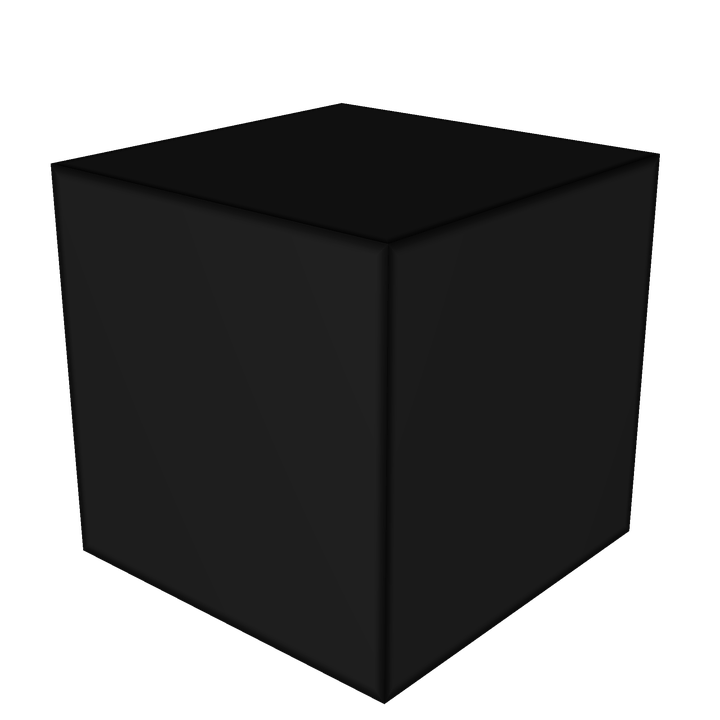
\includegraphics[width=106.5pt,height=104.25pt]{w07_hpo_grey_box/images/intro/black_box.png}};

% Text Node
\draw (284,106.5) node   [align=left] { \textcolor[rgb]{1,1,1}{{\Huge ?}}};
% Text Node
\draw (39,104) node   [align=left] {\textcolor[rgb]{1,1,1}{X}};
% Text Node
\draw (586,102) node   [align=left] {\textcolor[rgb]{1,1,1}{f(X)}};
% Text Node
\draw (317,28) node   [align=left] {Objective function};
% Text Node
\draw (309,254) node   [align=left] {Only interaction: Query of function at $\displaystyle \conf$ to obtain $\displaystyle \cost(\conf)$};


\end{tikzpicture}

\end{figure}
\pause
\begin{itemize}
    \item Can we do better?
\end{itemize}
\source{Peter Frazier: Grey-box Bayesian Optimization for AutoML ICML}
    
\end{frame}
%-------------------------------------------------
%-------------------------------------------------
\begin{frame}{Looking inside the box}
\begin{figure}
    \centering
    


\tikzset{every picture/.style={line width=0.75pt}} %set default line width to 0.75pt        

\begin{tikzpicture}[x=0.70pt,y=0.70pt,yscale=-1,xscale=1]
%uncomment if require: \path (0,300); %set diagram left start at 0, and has height of 300

%Straight Lines [id:da5075678478287002] 
\draw    (74.5,104) -- (218.5,104) ;
\draw [shift={(220.5,104)}, rotate = 180] [color={rgb, 255:red, 0; green, 0; blue, 0 }  ][line width=0.75]    (10.93,-3.29) .. controls (6.95,-1.4) and (3.31,-0.3) .. (0,0) .. controls (3.31,0.3) and (6.95,1.4) .. (10.93,3.29)   ;
%Shape: Square [id:dp6368535923226633] 
\draw  [fill={rgb, 255:red, 0; green, 25; blue, 255 }  ,fill opacity=1 ] (14,79) -- (64,79) -- (64,129) -- (14,129) -- cycle ;
%Shape: Square [id:dp8011400143211207] 
\draw  [fill={rgb, 255:red, 0; green, 25; blue, 255 }  ,fill opacity=1 ] (561,79) -- (611,79) -- (611,129) -- (561,129) -- cycle ;
%Straight Lines [id:da6772752516220095] 
\draw    (401.5,101) -- (540.5,101.99) ;
\draw [shift={(542.5,102)}, rotate = 180.41] [color={rgb, 255:red, 0; green, 0; blue, 0 }  ][line width=0.75]    (10.93,-3.29) .. controls (6.95,-1.4) and (3.31,-0.3) .. (0,0) .. controls (3.31,0.3) and (6.95,1.4) .. (10.93,3.29)   ;
%Straight Lines [id:da7102938160527976] 
\draw    (39.5,242) -- (39.01,143) ;
\draw [shift={(39,141)}, rotate = 449.72] [color={rgb, 255:red, 0; green, 0; blue, 0 }  ][line width=0.75]    (10.93,-3.29) .. controls (6.95,-1.4) and (3.31,-0.3) .. (0,0) .. controls (3.31,0.3) and (6.95,1.4) .. (10.93,3.29)   ;
%Straight Lines [id:da5275375794470956] 
\draw    (39.5,242) -- (123.5,242) ;
%Straight Lines [id:da11206880859629287] 
\draw    (123.5,242) -- (586.5,242) ;
%Straight Lines [id:da8957848321230528] 
\draw    (586.5,135) -- (586.5,242) ;
%Image [id:dp9410017568713034] 
\draw (307.5,95) node  {
\includegraphics[width=94.5pt,height=76.5pt]{w07_hpo_grey_box/images/intro/opened_box.png}};
%Straight Lines [id:da7498039648909043] 
\draw    (264,72) -- (222.18,45.08) ;
\draw [shift={(220.5,44)}, rotate = 392.77] [color={rgb, 255:red, 0; green, 0; blue, 0 }  ][line width=0.75]    (10.93,-3.29) .. controls (6.95,-1.4) and (3.31,-0.3) .. (0,0) .. controls (3.31,0.3) and (6.95,1.4) .. (10.93,3.29)   ;

% Text Node
\draw (39,104) node   [align=left] {\textcolor[rgb]{1,1,1}{X}};
% Text Node
\draw (586,102) node   [align=left] {\textcolor[rgb]{1,1,1}{f(X)}};
% Text Node
\draw (317,28) node   [align=left] {Objective function};
% Text Node
\draw (309,254) node   [align=left] {Only interaction: Query of function at $\displaystyle \conf$ to obtain $\displaystyle \cost(\conf)$};
% Text Node
\draw (158,38) node   [align=left] {other information};


\end{tikzpicture}

\end{figure}
\source{Peter Frazier: Grey-box Bayesian Optimization for AutoML ICML}
\end{frame}
%-------------------------------------------------
%-------------------------------------------------
\begin{frame}{Looking inside the box}
Utilize additional knowledge available about the objective function to improve optimization performance:
\begin{itemize}
    \item Learning curves:
    \begin{itemize}
        \item Early stopping
        \item Freezing \& Thawing
    \end{itemize}
    \item Cheap-to-evaluate proxies
    \begin{itemize}
        \item Trained neural network on small part of $\dataset$ 
    \end{itemize}
    \item Multi-task learning
    \begin{itemize}
        \item Solve multiple learning tasks simultaneously.
        \item Exploit commonalities and differences across tasks.
    \end{itemize}
    \item Warm starts
    \begin{itemize}
        \item Reuse trained hyperparameter configurations from similar models or datasets.
    \end{itemize}
\end{itemize}
\end{frame}
%-------------------------------------------------
%-------------------------------------------------
\iffalse
\begin{frame}{Learning Curves}

\centering
\includegraphics[width=0.4\textwidth]{w07_hpo_grey_box/images/intro/learning_curves.png}

Exemplary learning curves of training deep neural networks\\
Many ML algorithms iteratively optimize a (loss) function

\end{frame}
%-------------------------------------------------
%-------------------------------------------------
\begin{frame}{Stopping poor evaluations early}

\centering
\includegraphics[width=0.5\textwidth]{w07_hpo_grey_box/images/intro/differetiatingConfigurations.png}

Only stop evaluations after they have spent sufficient resources to differentiate between them in terms of quality.

\end{frame}
\fi
\section{Learning Curves}
\begin{frame}{Learning Curves}

\centering
\includegraphics[width=0.4\textwidth]{w07_hpo_grey_box/images/learningcurve/learning_curves.png}

Exemplary learning curves of training deep neural networks\\
Many ML algorithms iteratively optimize a (loss) function

\end{frame}
%-----------------------------------------------------------------------

%-----------------------------------------------------------------------
\begin{frame}{Learning Curve Predictions}

\centering
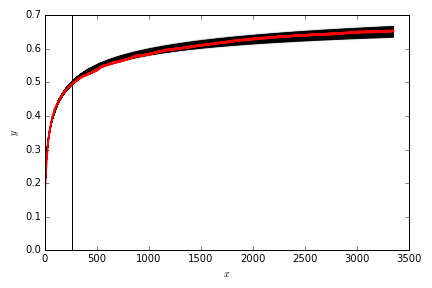
\includegraphics[width=0.5\textwidth]{w07_hpo_grey_box/images/learningcurve/learning_curve_single_pred.jpg}

\begin{enumerate}
  \item Observe learning curve for the first $n$ steps (here $n=250$)
  \pause
  \item \alert{Extrapolation}: fit parametric model on partial learning curve to predict remaining learning curve
  \pause
  \begin{itemize}
      \item Various models can be used (see following slides) 
  \end{itemize}
  
 % Which model to use? E.g.,
 % \begin{itemize}
%	\item Parametric density models: give table with equations
%	\item Neural network with learning curve layer
%	\item Recurrent neural network
%%    \item Good model depends on shape of curve $\to$ e.$\,$g., depends on optimizer  
%%    \item[$\leadsto$] combination of several models
%  \end{itemize}
  
\end{enumerate}

\end{frame}
%-----------------------------------------------------------------------

%-----------------------------------------------------------------------
\begin{frame}{Learning Curves: Early Termination}

\centering
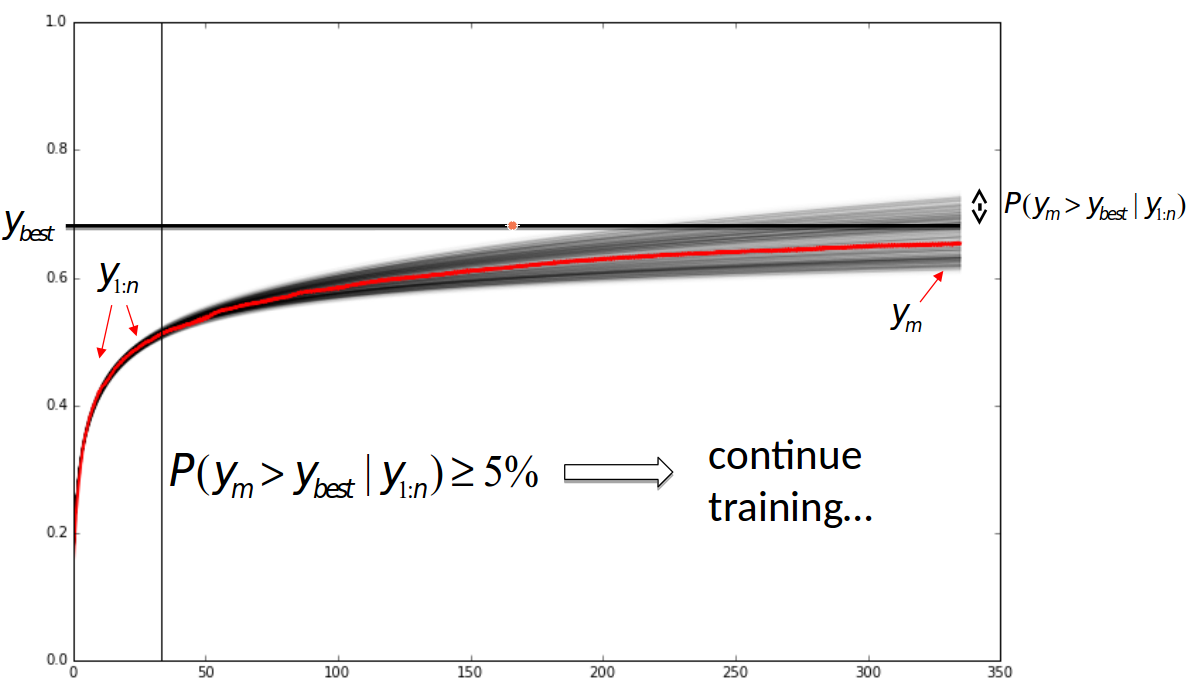
\includegraphics[width=0.8\textwidth]{w07_hpo_grey_box/images/learningcurve/learning_curve_dec.png}

$\rightarrow$ need for \alert{probabilistic predictions / quantification of uncertainty}

\end{frame}
%-----------------------------------------------------------------------
%-----------------------------------------------------------------------
\begin{frame}{Learning Curves: Early Termination}

\centering
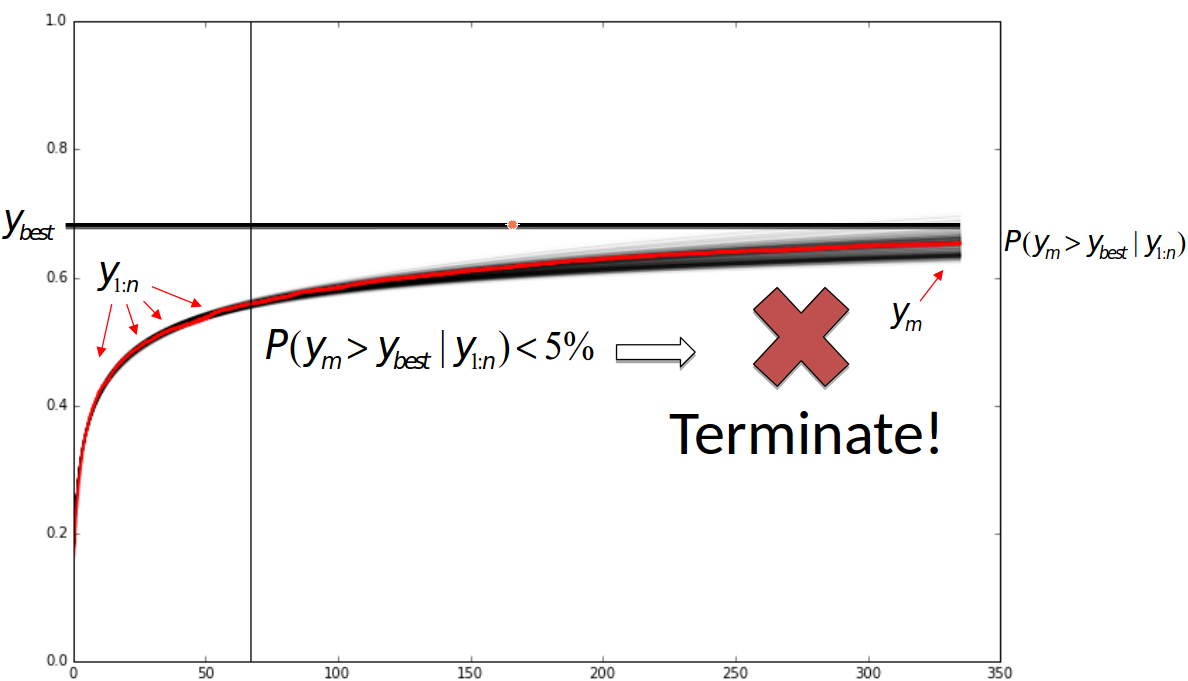
\includegraphics[width=0.8\textwidth]{w07_hpo_grey_box/images/learningcurve/learning_curve_dec2.png}

$\rightarrow$ need for \alert{probabilistic predictions / quantification of uncertainty}

\end{frame}
%-----------------------------------------------------------------------

%-----------------------------------------------------------------------
\begin{frame}{Parametric Learning Curves}

\myit{
	\item Use a parametric model $f_k$ with parameters $\boldsymbol{\theta}$ to model performance at step $t$ as:
	\alert{$y_t = f_k(t|\boldsymbol{\theta}) + \epsilon$}, with $\epsilon \sim \mathcal{N}(0, \sigma^2)$.
\pause
	\item Linear combination of $K=11$ parametric types of models:
	\alert{$f_{comb}(t|\bm{\xi}) = \sum_{k=1}^K w_k f_k(t|\boldsymbol{\theta}_k)$},
where $\bm{\xi} = (w_1, \dots, w_{K}, \boldsymbol{\theta}_1, \dots, \boldsymbol{\theta}_{K}, \sigma^2)$
%	\item MSc Thesis in my group, 2015
}
\begin{center}
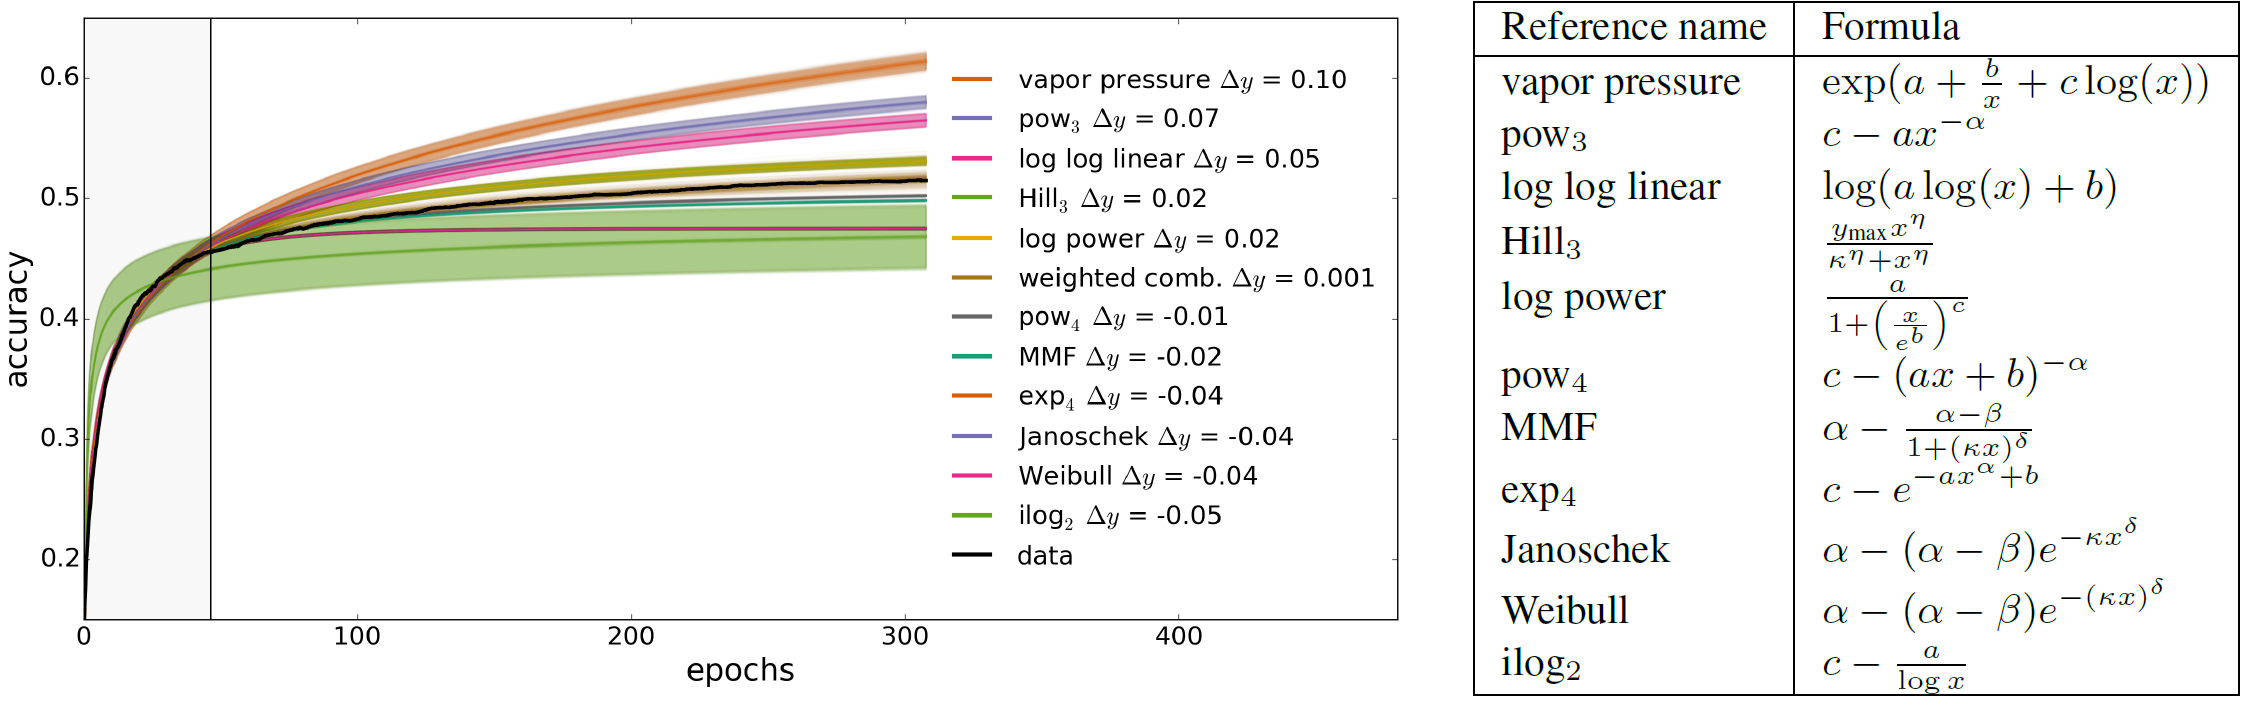
\includegraphics[width=0.9\textwidth]{w07_hpo_grey_box/images/learningcurve/Domhan_types_of_curves.png}\\
\scriptsize{$K=11$ parametric families for modelling learning curves}
\end{center}

\pause
\myit{
	\item Use Markov Chain Monte Carlo sampling of $\bm{\xi}$ to obtain uncertainties
}

\end{frame}
%-----------------------------------------------------------------------

%-----------------------------------------------------------------------
\begin{frame}{Predictive Termination}

{
\begin{center}
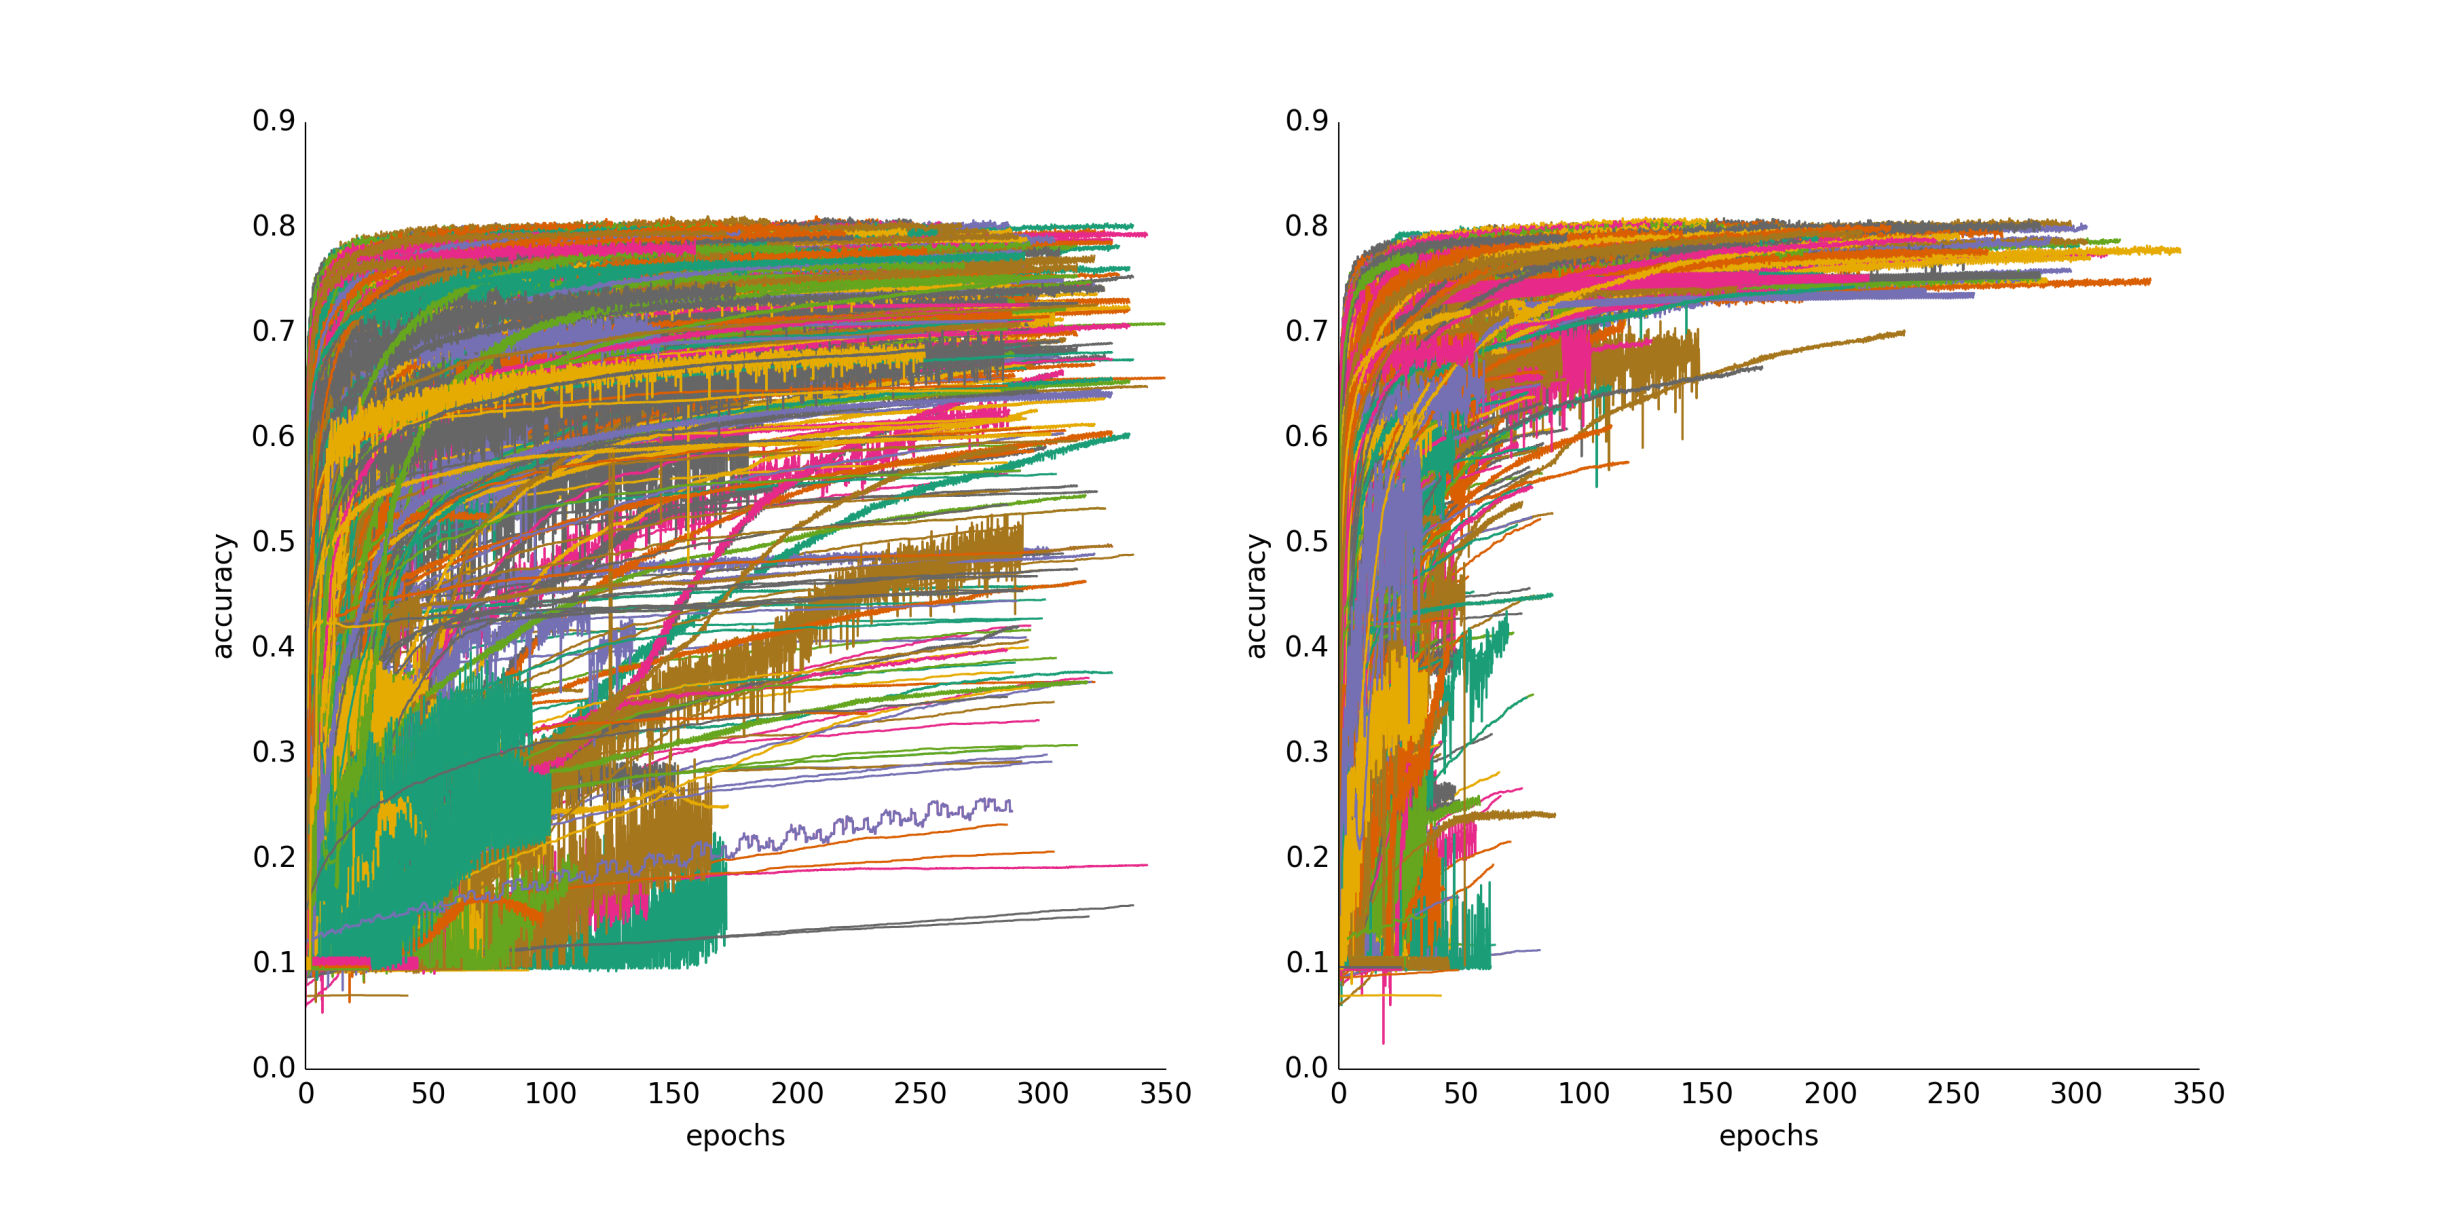
\includegraphics[width=0.9\textwidth]{w07_hpo_grey_box/images/learningcurve/learning_curve_tuning.jpg}

All learning curves vs. learning curves with early termination
\end{center}
}




\end{frame}
%-----------------------------------------------------------------------
%-----------------------------------------------------------------------
\begin{frame}{Predictive Termination}

{
\begin{center}
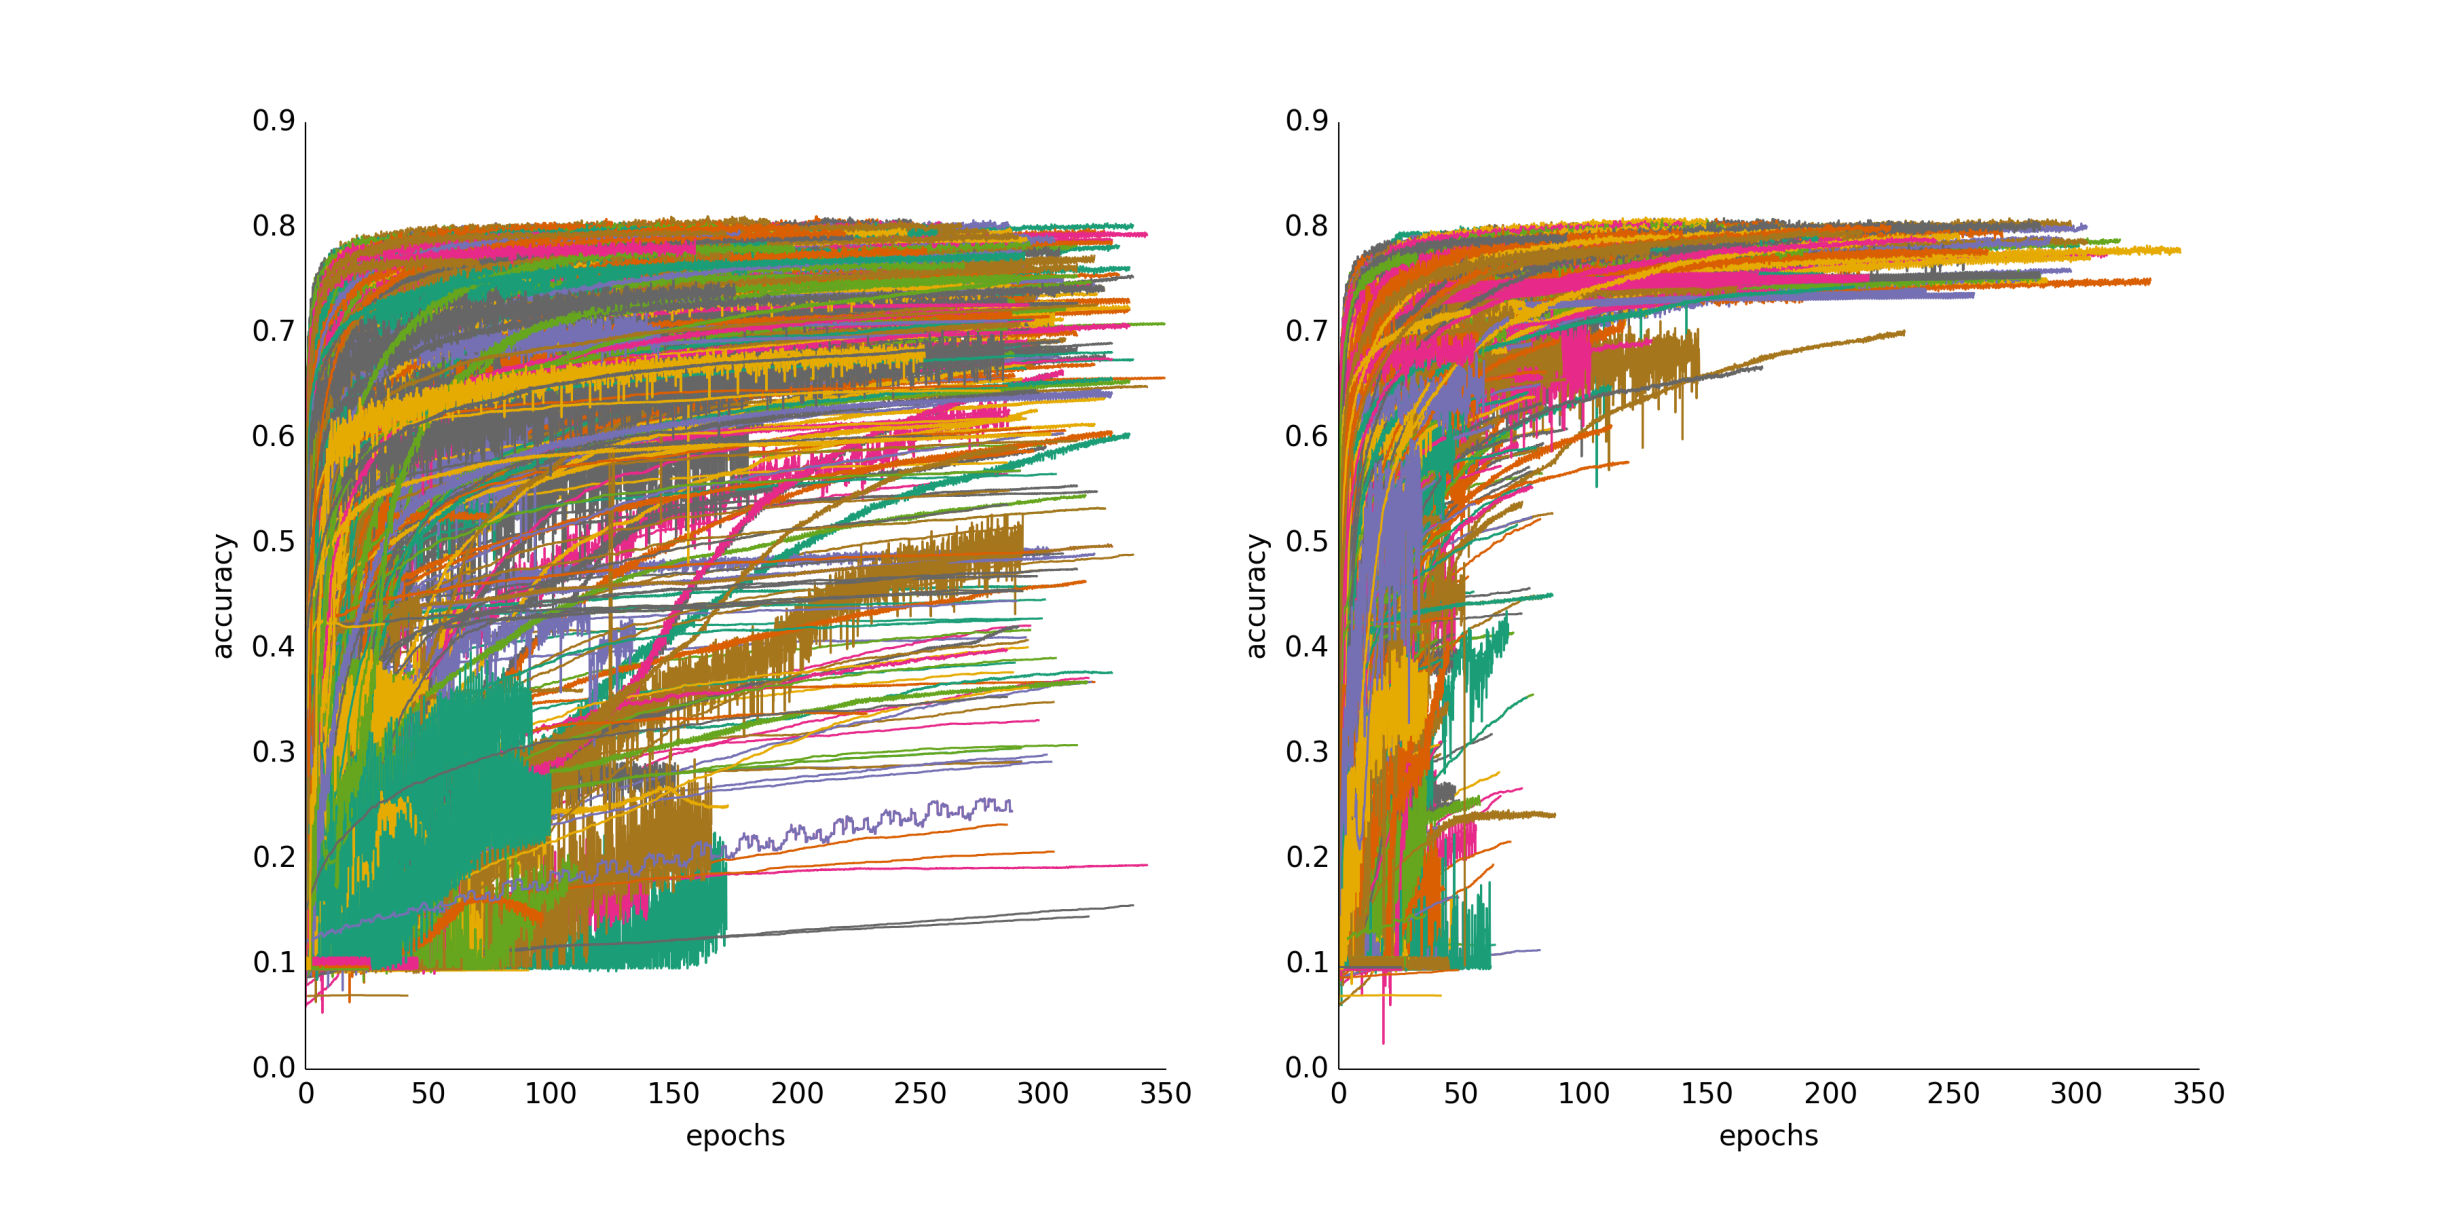
\includegraphics[width=0.5\textwidth]{w07_hpo_grey_box/images/learningcurve/learning_curve_tuning.jpg}

All learning curves vs. learning curves with early termination
\end{center}
}
\myit{
	\item Disadvantages of this model?
\pause
	\myit{
		\item Relies on manually-selected parametric families of curves
		\item Does not take into account hyperparameters used 
		\myit{
			\item[$\rightarrow$] can't learn across hyperparameters
		}
		\item Does not even learn across curves; simply extrapolates one at a time
%		\item Cannot quickly integrate new information from extending the curve
	}
}

\end{frame}
%-----------------------------------------------------------------------
\begin{frame}{Freeze-Thaw Bayesian Optimization}

\myit{
	\item Use a Gaussian process with inputs $\conf$ and $t$; special kernel for $t$
	\item For $N$ configurations and $T$ epochs each: $O(N^3 t^3)$ $\rightarrow$ approximation
	\item Iteratively: either extend existing configuration or try new one
\pause
	\item Result for probabilistic matrix factorization:
	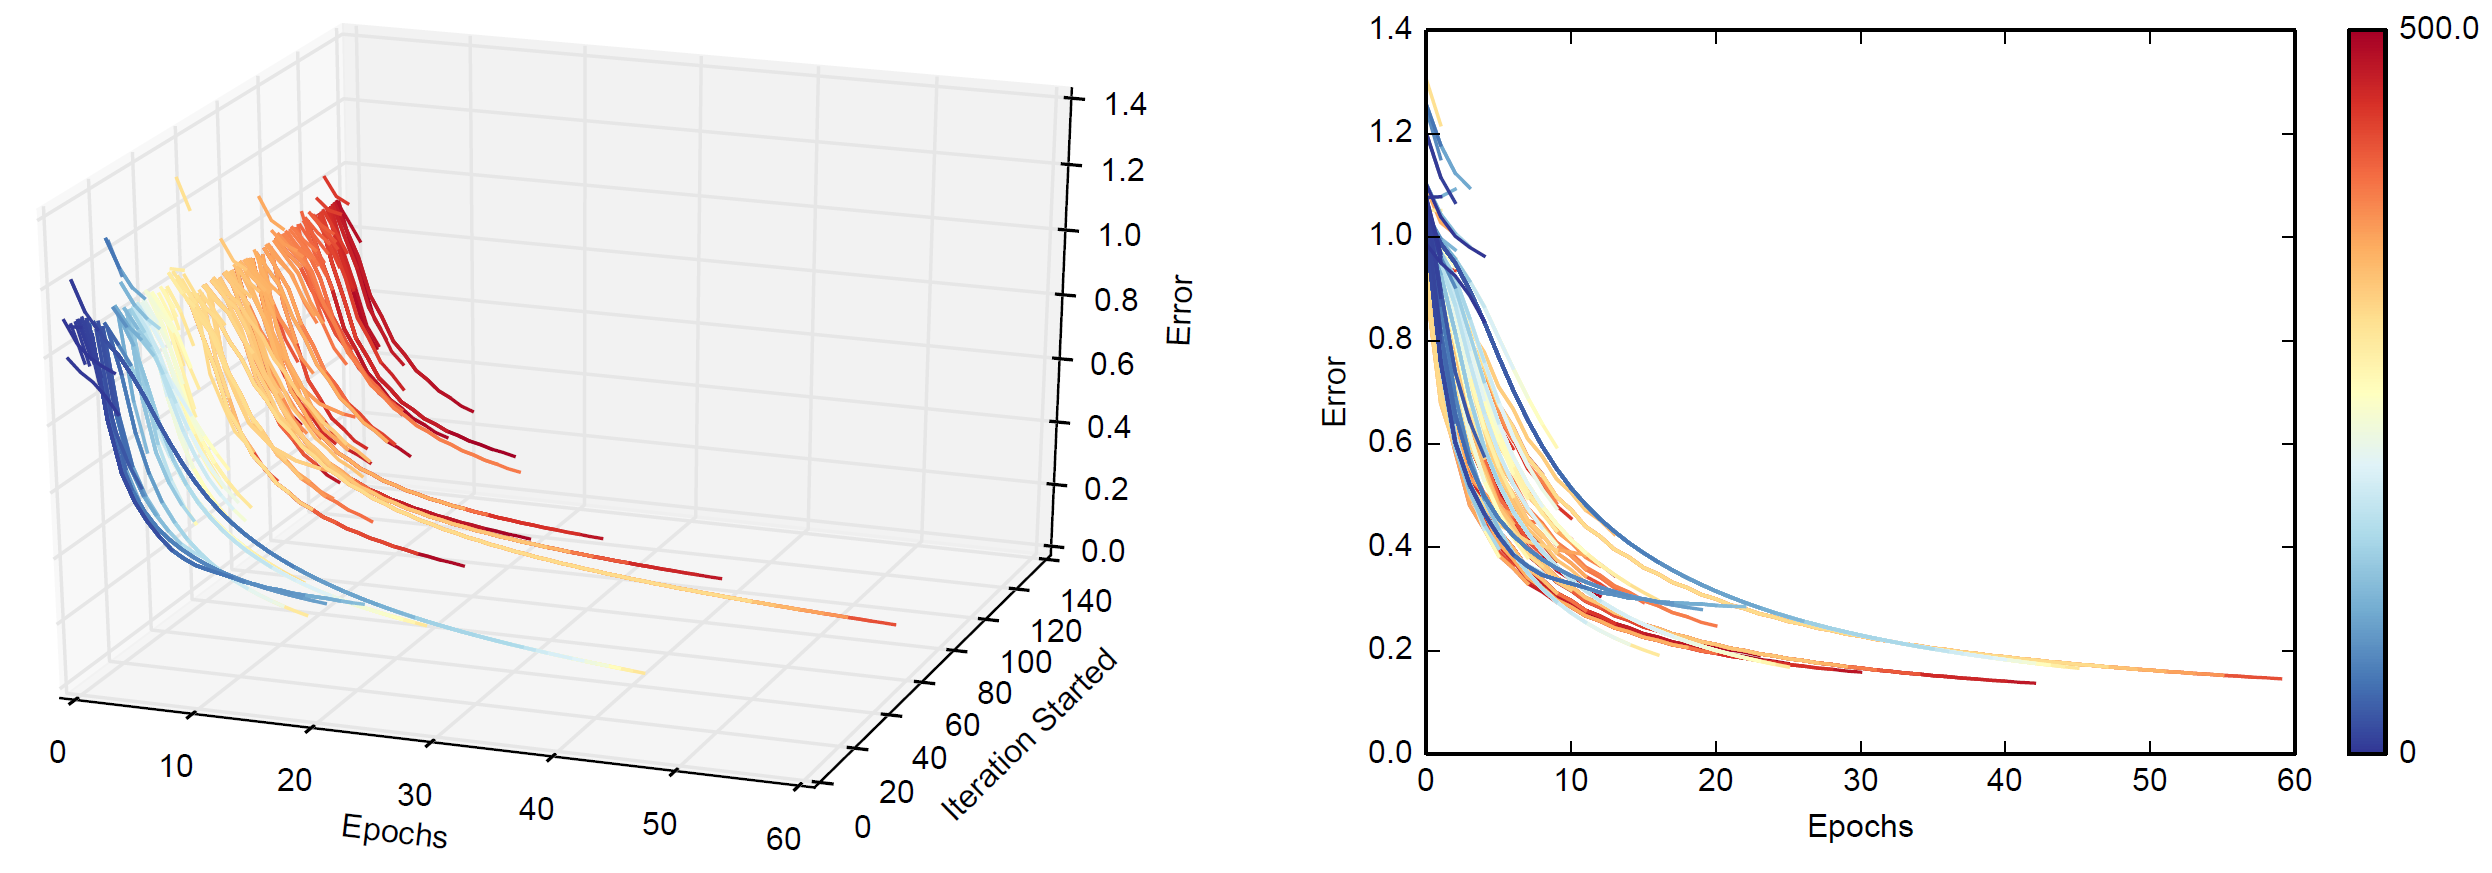
\includegraphics[width=0.8\textwidth]{w07_hpo_grey_box/images/learningcurve/FTBO.png}
\pause
	\item Unfortunately, no results for DNNs; no code available
}


\end{frame}
%-----------------------------------------------------------------------


%-----------------------------------------------------------------------
\begin{frame}{LC-Net}

\vspace*{-0.25em}
{
	\rightimage[.4]{w07_hpo_grey_box/images/learningcurve/LC-Net-network.png}
	\myit{
		\item \goleft[.45]{Make a layer out of the parametric learning curves by Domhan et al.}
		\item \goleft[.45]{Also support hyperparameters as inputs (in the figure denoted by $x_1, \dots, x_d$)}
%		\item \goleft[.45]{Work by my Phd student Aaron Klein and postdoc Stefan Falkner}
	}
}

\pause
\myit{
	\item Disadvantages of this model?
	\pause
	\myit{
		\item \goleft[.45]{Relies on manually-selected parametric families of curves}
		\item \goleft[.45]{Cannot quickly integrate new information from extending the current curve \\ (or from new runs)}
	}
}
\end{frame}
%-----------------------------------------------------------------------



%-----------------------------------------------------------------------
\begin{frame}{Sequence Models {\smaller{(e.g., Bayesian RNN)}}}

	\myit{
		\item Learning curves are \alert{sequences}
		\myit{
			\item Previous models don't treat them like this
			\item We can use an RNN (in particular, an LSTM) to predict the next value from a given sequence
			\item We can use variational dropout to obtain uncertainty estimates:
\pause
		}
	}

\begin{center}
	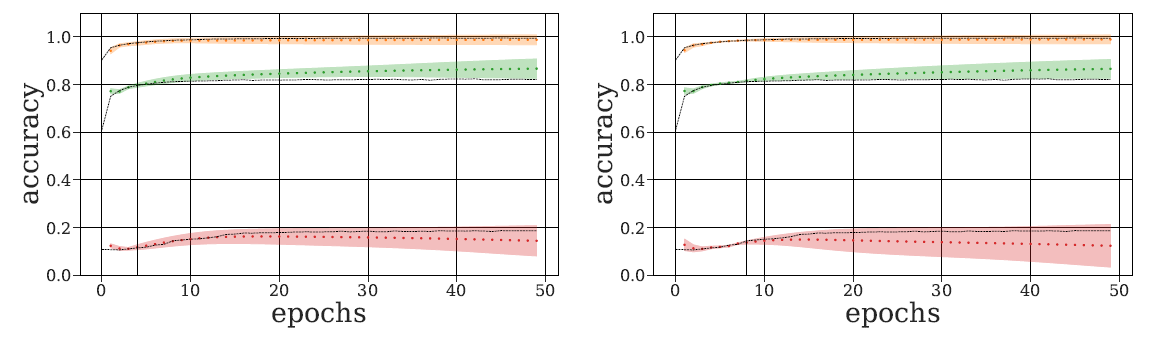
\includegraphics[width=0.58\textwidth]{w07_hpo_grey_box/images/learningcurve/Gargiani-MNIST-extrapolations_1.png}\\
	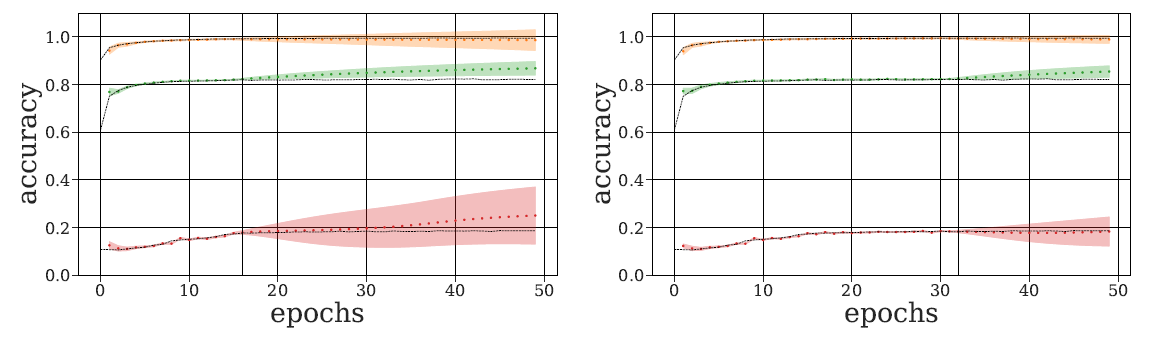
\includegraphics[width=0.58\textwidth]{w07_hpo_grey_box/images/learningcurve/Gargiani-MNIST-extrapolations_2.png}\\
\end{center}	
	
\end{frame}
%-----------------------------------------------------------------------
%-----------------------------------------------------------------------
\begin{frame}{Sequence Models {\smaller{(e.g., Bayesian RNN)}}}

	\myit{
		\item Note: we can also use a simpler model
		\myit{
			\item E.g., a random forest to map from a fixed-size window to the next value
		}
	}
\begin{center}
	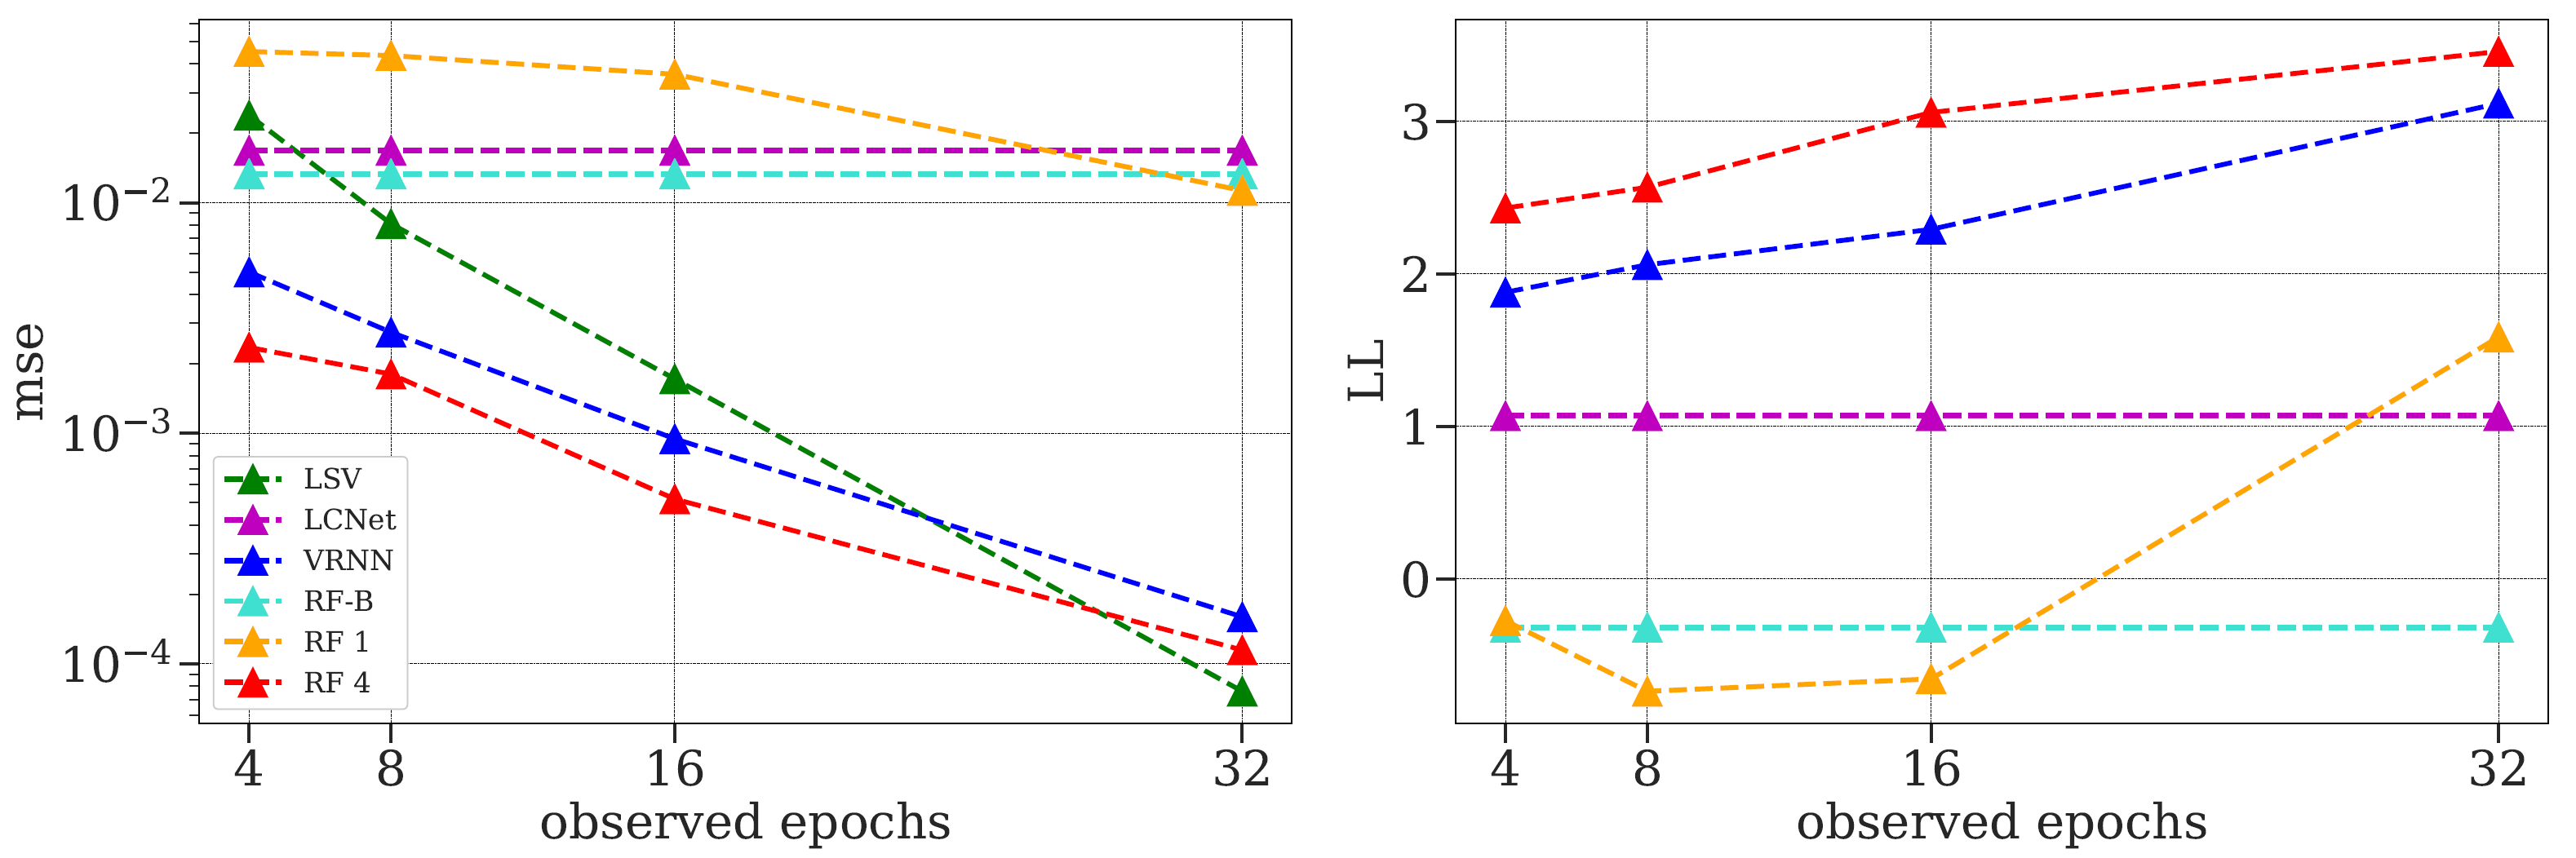
\includegraphics[width=0.9\textwidth]{w07_hpo_grey_box/images/learningcurve/Gargiani-MNIST-extrapolation-quality-based-on-different-sized-prefixes.png}
\end{center}	
\end{frame}
%-----------------------------------------------------------------------
%-----------------------------------------------------------------------
\begin{frame}{Compare: Baker et al, 2017}

	\myit{
		\item Idea: Map from configurations (including architectural hyperparameters) 
		and partial learning curves to the final performance

		\item Advantages
		\myit{
			\item \alert{Much simpler idea} than all the approaches just discussed: no need to model the entire learning curve
			\item \alert{Much easier to implement}
		}
		\item Disadvantage? \pause
		\alert{$\rightarrow$ requires many (e.g., 100) fully-evaluated learning curves as training data}
		\myit{
			\item After 100 full function evaluations we want to be pretty much converged in practice
			\item But definitely helpful for speeding up RL
			
		}
	}

%Describe simple idea, and how that works extremely well when you have a budget of 10.000 of function evaluations.

\end{frame}
%-----------------------------------------------------------------------


\myframe{Possible extension of LC models waiting to be done}{
	\myit{
		\item We could keep track of additional information to feed to our model for better predictions
		\myit{
			\item E.g., training \& validation cross-entropy loss \& accuracy
			\myit{
				\item Instead of only validation accuracy
			}
			\item E.g., split cross-entry into data-dependent \& weight dependent parts
			\item E.g., keep track of gradient norms, activation statistics, \ldots
		}
		\item Information about learning rate (\& weight decay) at each step
		\begin{itemize}
		    \item Only Predictive termination leads to a practically usable algorithm
		\end{itemize}
		
	}
}
\section{Tree-Parzen Estimator}
%-----------------------------------------------------------------------
%-----------------------------------------------------------------------
\begin{frame}[c]{Connection TPE-grey-box}

\comment{What should be the motivation for including TPE here? Just as an alternative for BO?}    

\end{frame}
%-----------------------------------------------------------------------
%-----------------------------------------------------------------------
\begin{frame}[c]{Tree-Parzen Estimator}

\begin{itemize}
	\item Assume that we already observed some configuration and the corresponding loss $D = \{(\conf_i, \boobs_i))\}_{i=1}^N$
	\begin{itemize}
		\item let's use $\boobs_i = f(\lambda)$ as a short form for $\mathcal{L}(\algo_{\conf}, \dataset_{train}, \dataset_{valid})$
	\end{itemize}
	\pause
	\item We could approximate the good and the bad regions of the configuration space $\pcs$
\end{itemize}

$$
p(\conf|y) = \begin{cases}
l(\conf) \text{ if } \boobs < \boobs^*\\
g(\conf) \text{ otherwise} 
\end{cases}
$$

where 
\begin{itemize}
	\item $\boobs^*$ is an empirical threshold for a well-performing configuration\\ (e.g., a $\gamma$ percentile of all observed $\boobs$ in $D$)
	\pause
	\item $l(\conf)$ models the density of the well-performing region based on $D$
\note[item] Note that we minimize!
	\pause
	\item $g(\conf)$ models the density of the poorly performing region based on $D$
	\pause
	\item $g$ and $l$ can be modeled by kernel density estimator (KDE)
\end{itemize}

\source{Bergstra et al. 2011}

\end{frame}
%-----------------------------------------------------------------------
%-----------------------------------------------------------------------
\begin{frame}[c]{Optimization with Tree-Parzen Estimator}
\begin{center}
\begin{minipage}{0.75\textwidth}
\begin{algorithm}[H]
    \LinesNumbered
    \SetAlgoLined
    \setcounter{AlgoLine}{0}
	\Input{Configuration Space $\pcs$,
		black box function $f$,
		maximal number of function evaluations $m$,
		percentile $\gamma$
	}
	\BlankLine
	$D_0$ $\leftarrow$ initial\_design($\pcs$); 
	\pause
	
	\For{\bocount = $1, 2, \ldots \bobudget - |\dataset_0|$}{
		$\dataset_\text{good}, \dataset_\text{bad}$ $\leftarrow$ Split $\dataset_{\bocount-1}$ into good and bad observations according to $\gamma$ percentile of all observed $\boobs$;
		\pause
		
		$l(\conf)$ $\leftarrow$ fit KDE on $\dataset_\text{good}$; 
		$g(\conf)$ $\leftarrow$ fit KDE on $\dataset_\text{bad}$;
		\pause
		
		$\Lambda_\text{cand}$ $\leftarrow$ draw examples according to $l$;
		\pause
		
		select $\conf_{\bocount}$ by optimizing $\conf_{\bocount} \in \argmax_{\conf \in \Lambda_\text{cand}} l(\conf) / g(\conf)$;
		\pause
		
		Query $\boobs_{\bocount} := \func(\lambda_{\bocount})$;
		
		Add observation to data $\dataset_{\bocount} := \dataset_{\bocount-1} \cup \{\langle \conf_{\bocount}, \boobs_{\bocount} \rangle \}$;
	}
	\Return{Best observed $\lambda$ according to $\dataset_\bobudget$}
	\caption{Optimization with TPE}
\end{algorithm}
\end{minipage}
\end{center}

\source{Bergstra et al. 2011}

\end{frame}
%-----------------------------------------------------------------------
%-----------------------------------------------------------------------
\begin{frame}[c]{Optimization with Tree-Parzen Estimator}

\centering
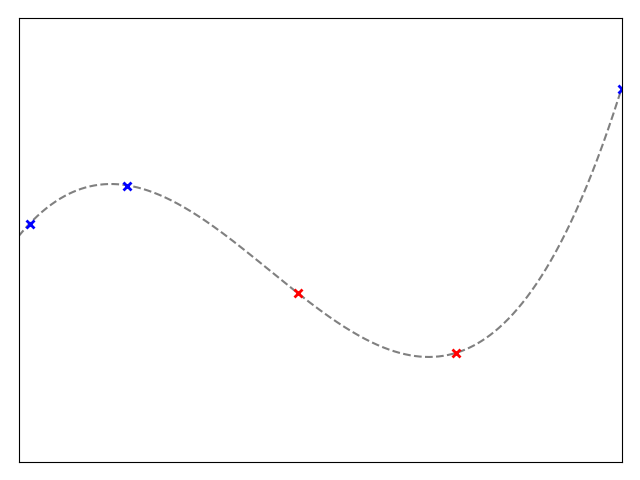
\includegraphics[width=0.6\textwidth]{w07_hpo_grey_box/images/tpe/tpeiter_1_observations.png}


\end{frame}
%-----------------------------------------------------------------------
%-----------------------------------------------------------------------
\begin{frame}[c]{Optimization with Tree-Parzen Estimator}

\centering
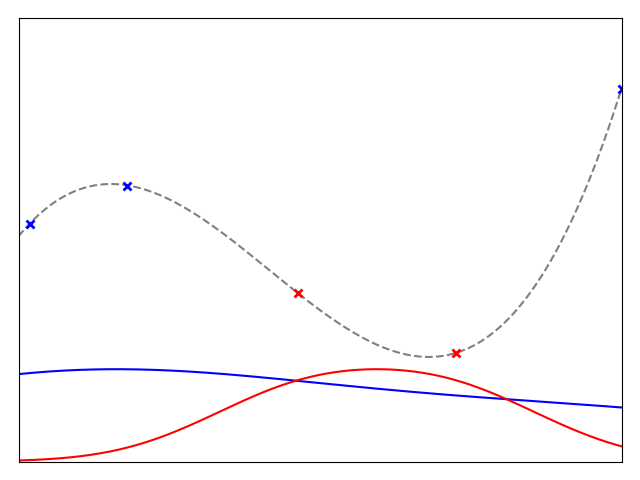
\includegraphics[width=0.6\textwidth]{w07_hpo_grey_box/images/tpe/tpeiter_1_pdfs.png}


\end{frame}
%-----------------------------------------------------------------------
%-----------------------------------------------------------------------
\begin{frame}[c]{Optimization with Tree-Parzen Estimator}

\centering
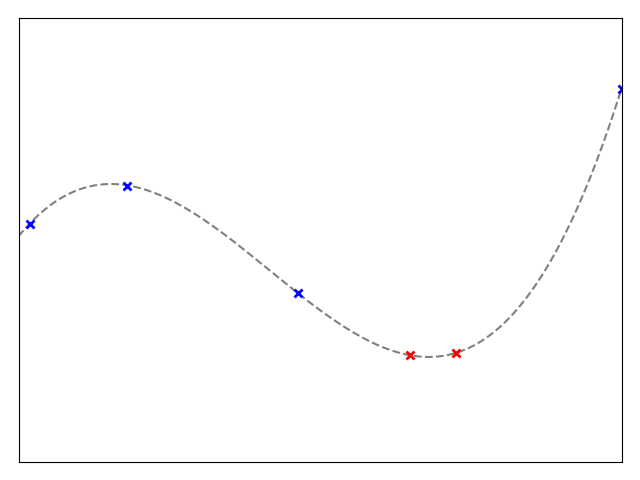
\includegraphics[width=0.6\textwidth]{w07_hpo_grey_box/images/tpe/tpeiter_2_observations.png}


\end{frame}
%-----------------------------------------------------------------------
%-----------------------------------------------------------------------
\begin{frame}[c]{Optimization with Tree-Parzen Estimator}

\centering
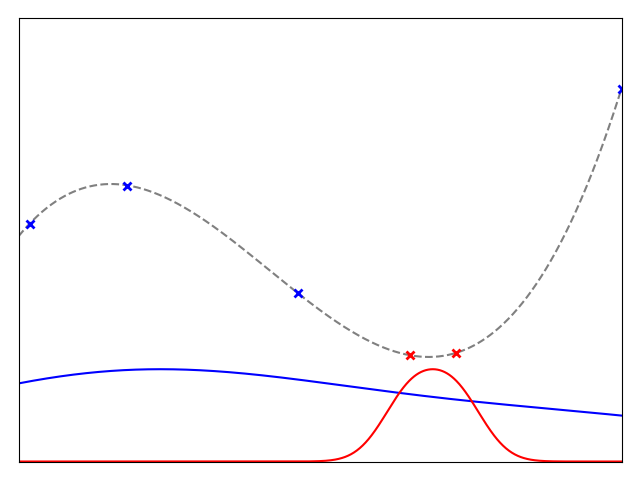
\includegraphics[width=0.6\textwidth]{w07_hpo_grey_box/images/tpe/tpeiter_2_pdfs.png}


\end{frame}
%-----------------------------------------------------------------------
%-----------------------------------------------------------------------
\begin{frame}[c]{Optimization with Tree-Parzen Estimator}

\centering
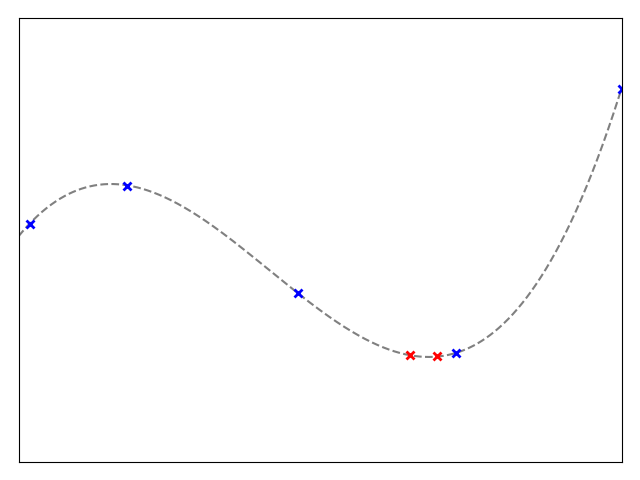
\includegraphics[width=0.6\textwidth]{w07_hpo_grey_box/images/tpe/tpeiter_3_observations.png}


\end{frame}
%-----------------------------------------------------------------------
%-----------------------------------------------------------------------
\begin{frame}[c]{Optimization with Tree-Parzen Estimator}

\centering
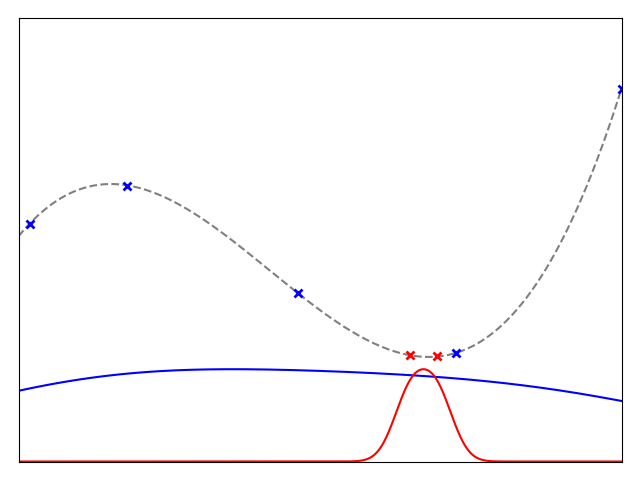
\includegraphics[width=0.6\textwidth]{w07_hpo_grey_box/images/tpe/tpeiter_3_pdfs.png}


\end{frame}
%-----------------------------------------------------------------------
%-----------------------------------------------------------------------
\begin{frame}[c]{Optimization with Tree-Parzen Estimator}


Remarks:

\begin{itemize}
	\item TPE models $p(\conf | \boobs)$
	\begin{itemize}
		\item we can multiply it with a prior to add expert knowledge
	\end{itemize}
	\smallskip
	\pause
	\item Performance of TPE depends on:
	\begin{itemize}
		\item setting of $\gamma$ to trade-off exploration and exploitation
		\item bandwidth of the KDEs 
	\end{itemize}
	\pause
	\smallskip
	\item optimizing $l(\conf)/g(\conf)$ is equivalent to optimizing \emph{expected improvement} as acquisition function in Bayesian Optimization
	\pause
	\smallskip
	\item successful tool implementing TPE is HyperOpt
\end{itemize}

\end{frame}
%-----------------------------------------------------------------------
%-----------------------------------------------------------------------
\begin{frame}[c]{Optimization with Tree-Parzen Estimator: Summary}
\begin{columns}[T] % align columns
\begin{column}{.48\textwidth}


    \begin{block}{Advantages}
    \begin{itemize}
    	\item Efficient $O(N*d)$
    	\pause
    	\item Parallelizable
    	\pause
    	\item Robust
    	\pause
    	\item Deal with complex search spaces with priors
    	\pause
    \end{itemize}
    \end{block}
\pause
\end{column}%

\hfill%

\begin{column}{.48\textwidth}

    \begin{block}{Disadvantages}
    \begin{itemize}
    	\item Less sample-efficient than GPs
    \end{itemize}
\end{block}

\end{column}
\end{columns}   

\end{frame}
%-----------------------------------------------------------------------
%-----------------------------------------------------------------------
	
\section{Meta-Learning}
%----------------------------------------------------------------------
%----------------------------------------------------------------------
\begin{frame}[c]{Meta-Learning: Introduction}

\begin{itemize}
	\item Learning essentially never stops:
	\begin{itemize}
		\item Many models are periodically re-fit to track changes in the data
		\item Many models are re-fit to perform well on new tasks
	\end{itemize}
	
    \item Learning is often done from scratch
    
    \item We humans do not start from scratch all the time \\ - we learned how to learn!
\end{itemize}

\end{frame}
%----------------------------------------------------------------------
%----------------------------------------------------------------------
\begin{frame}[c]{Meta-Learning: Introduction}

\begin{columns}
	\column{0.18\textwidth}
	Ren\'e Magritte
	\centering
	
\includegraphics[width=1.0\textwidth]{images/meta_learning/magritte_1.jpg}
	
\includegraphics[width=1.0\textwidth]{images/meta_learning/magritte_2.jpg}
	\column{0.258\textwidth}
	Francis Picabia
	\centering
	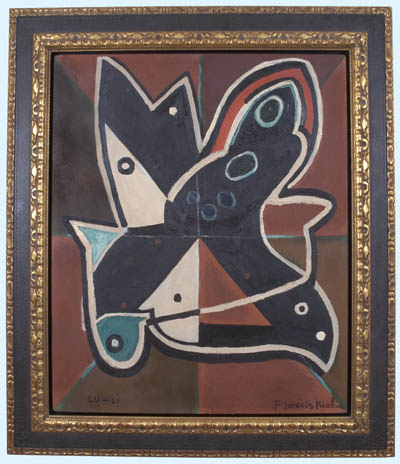
\includegraphics[width=.8\textwidth]{images/meta_learning/picabia_3.jpg}
	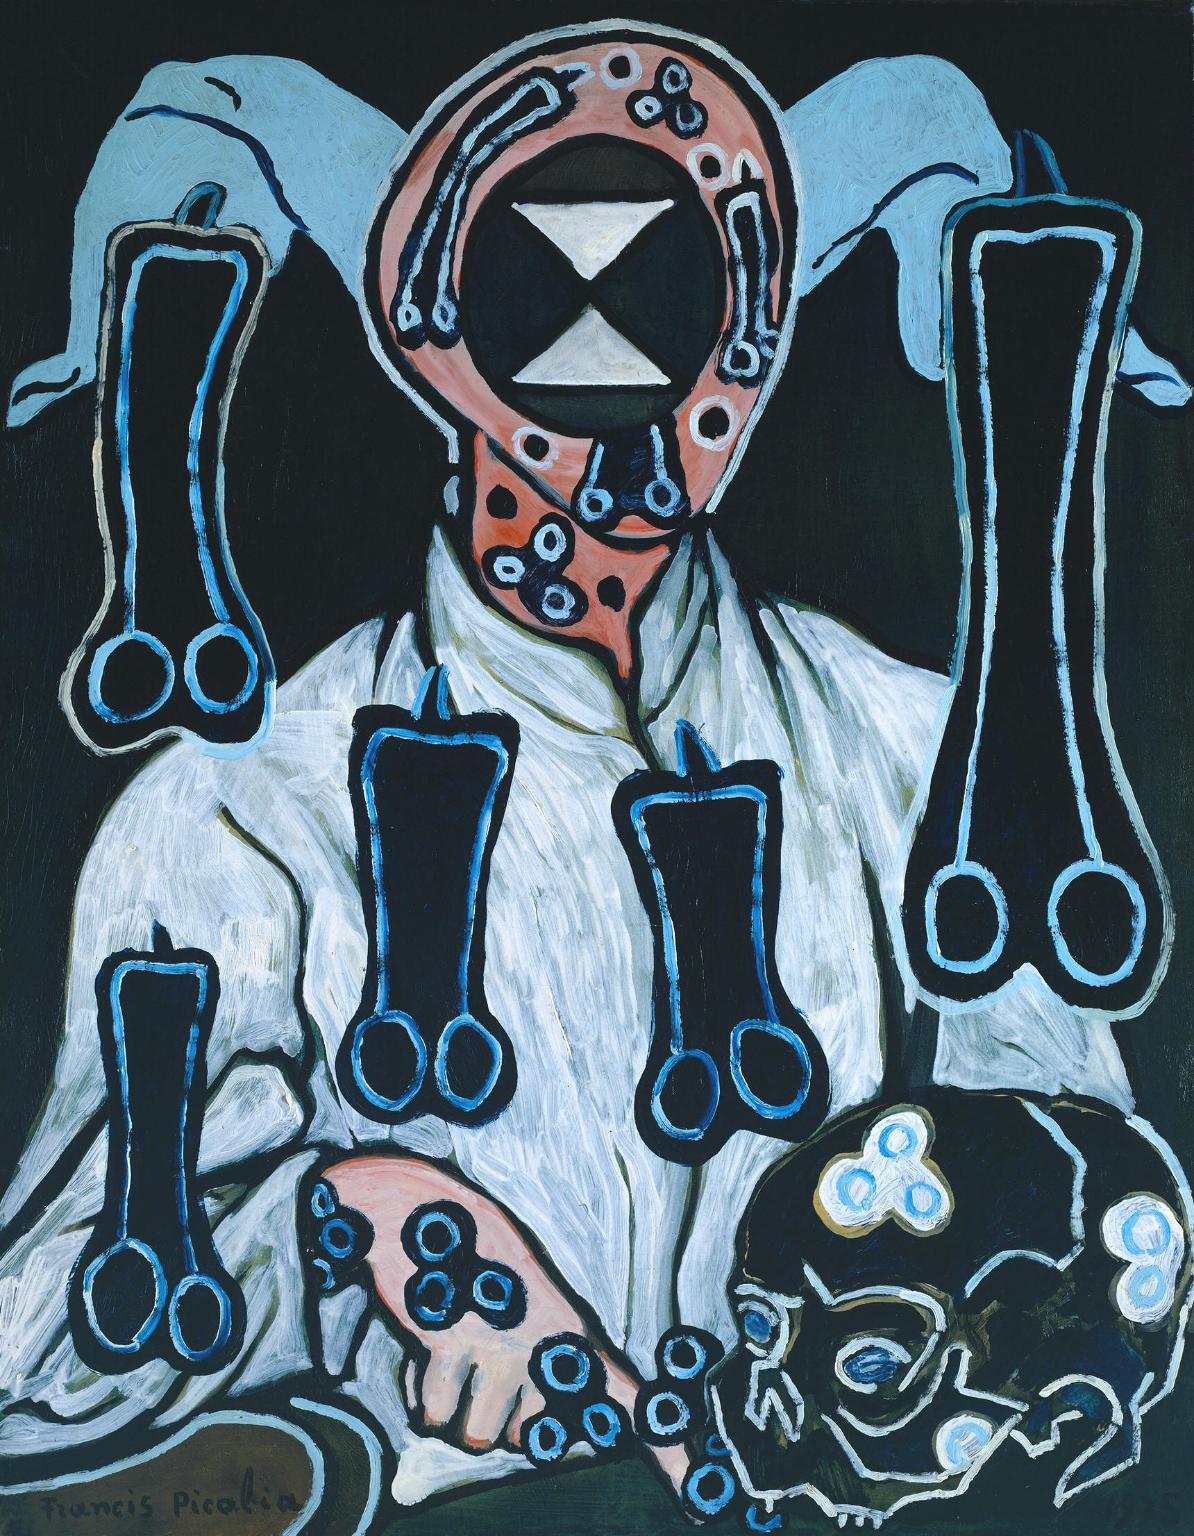
\includegraphics[width=.7\textwidth]{images/meta_learning/picabia_1.jpg}
	\column{0.3\textwidth}
	\centering
	Who painted that?
	
\includegraphics[width=.8\textwidth]{images/meta_learning/magritte_3.jpg}
	
	\pause
	Most likely most of you can identify the painter correctly, 
	although I presented only two pictures of each.
\end{columns}

\end{frame}
%----------------------------------------------------------------------
%----------------------------------------------------------------------
\begin{frame}[c]{Meta-Learning: Supervised Learning revisited}

Dataset:
\begin{equation*}
\dataset = \{(x_1, y_1), \ldots, (x_k, y_k) \}
\end{equation*}

\bigskip
\pause

Learning a model $\phi$ (e.g., weights of a neural network):
\begin{eqnarray*}
\argmax_{\phi} \log p(\phi|\dataset)\\
\pause
= \argmax_{\phi} \log p(\dataset | \phi) + \log p(\phi) \\
\pause
= \argmax_{\phi} \sum_i \log p(y_i | x_i, \phi) + \log p(\phi)
\end{eqnarray*}

\pause

Challenge:
\begin{itemize}
	\item Learning starts from scratch
	\item We might only have very few examples in $\dataset$ 
\end{itemize}

\end{frame}
%----------------------------------------------------------------------
%----------------------------------------------------------------------
\begin{frame}[c]{Meta-Learning: Problem formulation}

Dataset:
\begin{equation*}
\dataset = \{(x_1, y_1), \ldots, (x_k, y_k) \}
\end{equation*}
Set of datasets (meta-datasets):
\begin{equation*}
\mdata = \{\mathcal{D}_1, \ldots, \mathcal{D}_n, \}
\end{equation*}

\pause
Can we include these meta-datasets to improve learning on $\dataset$?
\begin{equation*}
\argmax_{\phi} \log p(\phi|\dataset, \mdata)
\end{equation*}

\pause
\medskip

\alert{Idea:} Instead of keeping $\mdata$ forever, we want to distill the knowledge into \alert{meta-parameters $\theta$}: $p(\theta|\mdata)$
 
\end{frame}
%----------------------------------------------------------------------
%----------------------------------------------------------------------
\begin{frame}[c]{Meta-Learning: Problem formulation}

In meta-learning, we want to learn:
\begin{eqnarray*}
\argmax_{\phi} \log p(\phi|\dataset, \mdata) \\
\pause
= \argmax_{\phi} \log \int_{\Theta} p(\phi \mid \dataset, \theta) p(\theta \mid \mdata) d\theta\\
\pause
\approx \argmax_{\phi} \log p(\phi | \dataset, \theta^*) + \log p(\theta^* | \mdata)\\
\pause
= \argmax_{\phi} \log p(\phi | \dataset, \theta^*)
\end{eqnarray*}

\pause

\begin{center}
\begin{minipage}{0.5\textwidth}
\begin{block}{Meta-learning problem}
\begin{equation*}
\theta^* \in \argmax_{\theta} \log p(\theta | \mdata)
\end{equation*}
\end{block}
\end{minipage}
\end{center}

\end{frame}
%-----------------------------------------------------------------------
%-----------------------------------------------------------------------
\begin{frame}[c]{Meta-Learning: AutoML $\subset$ Meta-Learning}

\begin{itemize}
	\item AutoML can be seen as a special case of meta-learning \pause
	\medskip
	\item $\theta$ could be:
	\begin{itemize}
		\item a hyperparameter configuration ($\lambda$) 
		\item a neural network architecture
	\end{itemize}
	\pause
	\medskip
	\item What would be $\mdata$ here? 
	\pause
	\begin{itemize}
		\item A dataset on which we optimized $\lambda$ (e.g. CIFAR-10)\\ such that we can use it on another dataset (e.g. imagenet)
	\end{itemize}
\end{itemize}	

\end{frame}
%-----------------------------------------------------------------------
%-----------------------------------------------------------------------
\begin{frame}[c]{Meta-Learning: Meta-Learning $\subset$ AutoML}

\begin{itemize}
	\item Meta-learning can be powerful to complement AutoML
	\pause
	\medskip
	\item We can learn a lot of things from $\mdata$ to improve the performance on new datasets, e.g.:
	\begin{itemize}
		\item pre-initialization of networks weights
		\item learning a meta-DNN to predict how to train another target-DNN	\end{itemize}
\end{itemize}	

\end{frame}
%-----------------------------------------------------------------------
%-----------------------------------------------------------------------
\begin{frame}[c]{Meta-Learning: Meta-Features in Machine Learning}
	
Based on their types and underlying assumptions, meta-features can be divided into at least five groups:
\pause
\begin{itemize}
	\item \alert{Simple meta-features} - number of features, patterns or classes, describe the basic dataset structure. \pause
	\item \alert{PCA meta-features} - compute various statistics of the datasets principal components. \pause
	\item \alert{The information-theoretic meta-features} - measure the class
entropy in the data. \pause
	\item \alert{Statistical meta-features} - characterize the data via descriptive statistics (e.g. the kurtosis or the dispersion of the label distribution).\pause
	\item \alert{Landmarking meta-features} - computed by running several
fast machine learning algorithms on the dataset. Based on
their learning scheme they can capture different properties
of the dataset, like e.g. linear separability.
\end{itemize}

\end{frame}
%-----------------------------------------------------------------------
%-----------------------------------------------------------------------
\begin{frame}[c]{Meta-Learning: Warmstarting}
	
\begin{itemize}
	\item Recap: Instead of starting from a random configuration we often start from a expert-defined configuration for hyperparameter optimization (HPO)
	\pause
	\item We also know that the default configuration often does not perform well on a new dataset
	\begin{itemize}
		\item Otherwise there would be no point in HPO
	\end{itemize}
	\pause
	\item \alert{Can we learn from previous datasets $\mdata$ how to initialize HPO?}\\
	(i.e., running an initial design)
	\begin{itemize}
		\item the same ideas also apply to NAS
		\item for simplicity we focus on HPO 
	\end{itemize}
\end{itemize}

\end{frame}
%-----------------------------------------------------------------------
%-----------------------------------------------------------------------
\begin{frame}[c]{Meta-Learning: Warmstarting}
	
\comment{Should we include some graphs for warmstarting?}

\end{frame}
%-----------------------------------------------------------------------
%-----------------------------------------------------------------------
\begin{frame}[c]{Meta-Learning: Learning Acquisition Functions}

\begin{itemize}
	\item Instead of learning everything, it might be sufficient to \alert{learn hand-design heuristics}
	\pause
	\item In Bayesian Optimization (BO), the most critical hand-design heuristic is the acquisition function
	\begin{itemize}
		\item trade-off between exploitation and exploration
		\item Depending on the problem at hand, you might need a different acquisition function
		\pause
		\item Choices:
		\begin{itemize}
			\item probability of improvement (PI)
			\item expected improvement (EI)
			\item upper confidence bounds (UCB)
			\item entropy search (ES) 
			\item knowledge gradient (KG)
			\item ...
		\end{itemize} 
	\end{itemize}
	\pause
	\item \alert{Idea:} Learn a \emph{neural acquisition function} from data
\end{itemize}

$\leadsto$ Replace acquisition function 

\source{Volpp et al.'19}

\end{frame}
%-----------------------------------------------------------------------
%-----------------------------------------------------------------------
\begin{frame}[c]{Meta-Learning: Learning Acquisition Functions}
	
Although the \alert{acquisition function $\alpha$} depends on the history $\mathcal{D}_{\bocount-1}$ and the predictive model $\surro$, $\alpha$ mainly makes use of the \alert{predictive mean $\mu$ and variance $\sigma^2$}.

\pause
\bigskip

Neural acquisition function (AF):

\begin{eqnarray}
\acq_\theta(x) = \acq_\theta(\mu_t(x), \sigma_t(x)) \nonumber
\end{eqnarray}

where $\theta$ are the parameters of a neural network,\\ and $\mu$ and $\sigma$ are its inputs.

\pause 
\begin{itemize}
	\item Since the input is not $x$, it allows to learn scalable acquisition function
	\item No calibration of hyperparameter necessary, once the neural AF is learnt
\end{itemize}

\end{frame}
%-----------------------------------------------------------------------
%-----------------------------------------------------------------------
\begin{frame}[c]{Meta-Learning: Learning Acquisition Functions}
	
\comment{Do you want to include this topic? (I did so we can easily delete it)}

\end{frame}
%-----------------------------------------------------------------------
%-----------------------------------------------------------------------

%-----------------------------------------------------------------------
%-----------------------------------------------------------------------
\begin{frame}[c]{Meta-Learning: Task-independent recommendations}



\begin{columns}[T] % align columns
\begin{column}{.48\textwidth}

    \begin{itemize}
        \item<1-7> \emph{Idea:} learn a sorted list of defaults
        \item<2-7> \emph{Method:} mostly greedy 
        \item<3-7> \emph{Results:} improves over Random Search and Bayesian Optimization
    \end{itemize}

    \only<4-7>{
    \begin{block}{Advantages}
    \begin{itemize}
    	\item<4-7> Easy to share and use
    	\item<5-7> Strong anytime performance
    	\item<6-7> Embarrassingly parallel
    \end{itemize}
    \end{block}}
    
    \only<7-7>{
    \begin{block}{Disadvantages}
    \begin{itemize}
    	\item<7-7> Not adaptive
    \end{itemize}
    \end{block}}

\end{column}%

\hfill%

\begin{column}{.48\textwidth}

    \centering
    \only<1-2>{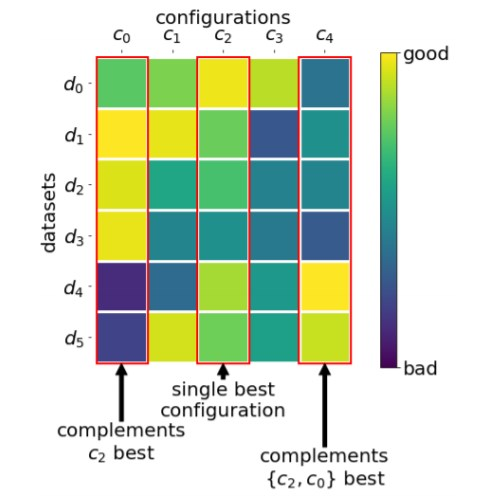
\includegraphics[width=.8\textwidth]{images/meta_learning/task_independent.jpg}}
    \only<3-7>{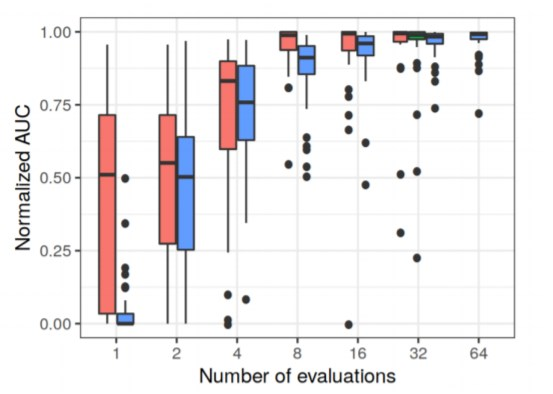
\includegraphics[width=.9\textwidth]{images/meta_learning/task_independent_results.jpg}}


\end{column}
\end{columns}  

\source{Wistuba et al., 2015a,\&b, Feurer et al., 2018, Pfisterer et al., 2018}

\end{frame}
%-----------------------------------------------------------------------
%-----------------------------------------------------------------------



%-----------------------------------------------------------------------
%-----------------------------------------------------------------------
\begin{frame}[c]{Meta-Learning: Joint model for Bayesian optimization}

\begin{columns}[T] % align columns
\begin{column}{.38\textwidth}

\begin{itemize}
    \item<1-5> Jointly train a „deep“ neural network on all tasks 
    \item<2-5> Have a separate output layer (head) for each tasks 
    \item<3-5> Each head is a Bayesian linear regression 
    \item<4-5> Feature extraction on hyperparameter configurations 
    \item<5-5> (Recall DNGO)
\end{itemize}
\end{column}%

\hfill%

\begin{column}{.58\textwidth}
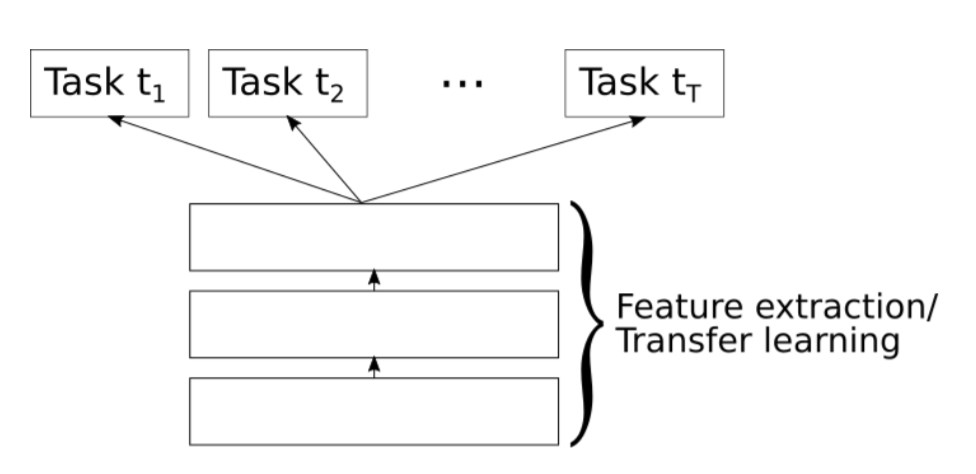
\includegraphics[width=0.9\textwidth]{images/meta_learning/perrone_int.jpg}
\end{column}%
\end{columns}

\source{Perrone et al. 2018}

\end{frame}
%-----------------------------------------------------------------------
%-----------------------------------------------------------------------
\begin{frame}[c]{Meta-Learning: Joint model for Bayesian optimization}
	
\centering
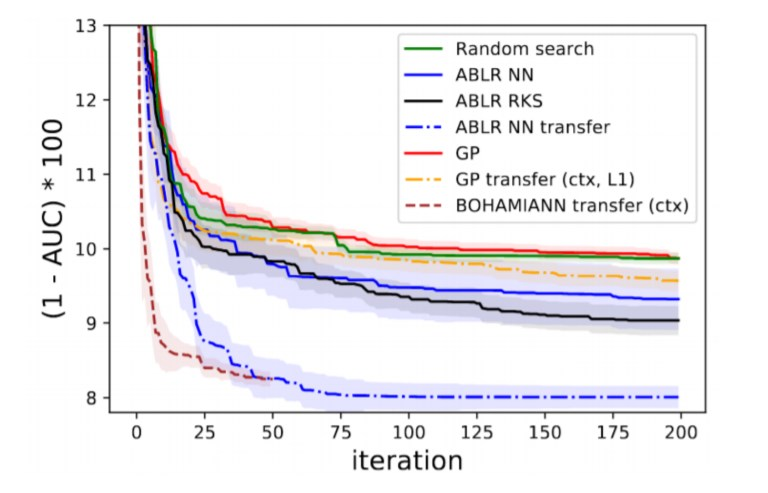
\includegraphics[width=0.7\textwidth]{images/meta_learning/perrone_res.jpg}

\end{frame}
%-----------------------------------------------------------------------
%-----------------------------------------------------------------------

%----------------------------------------------------------------------
\section{Hyperband}

%-----------------------------------------------------------------------

\begin{frame}{Bandit-Based Hyperparameter Optimization}
\begin{columns}[T]

\begin{column}{.45\textwidth}
    \begin{itemize}
        \item Idea: Allocate more resources to promising configurations, eliminate poor ones early.
        \pause
    \end{itemize}
\end{column}
    \begin{column}{.45\linewidth}
    \begin{figure}
    \centering
    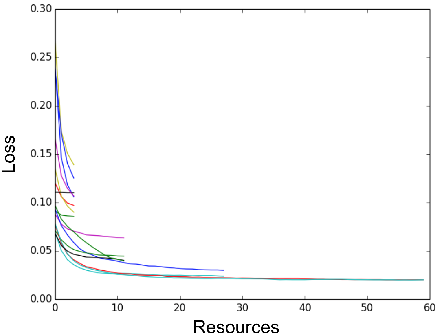
\includegraphics[width=0.9\linewidth]{w07_hpo_grey_box/images/hyperband/Figure_1_2.png}
\end{figure}
    \end{column}
    \end{columns}
    \begin{columns}
    
    \begin{column}{.45\linewidth}
    \vspace{-9em}
    \begin{itemize}
	\item Result: Examine more configurations.
	\pause
	\item Resources:
	\pause
	\begin{itemize}
	    \item Runtime
	    \pause
	    \item Number of epochs/iterations
	    \pause
	    \item Number of trees
	    \pause
	    \item Data subset size
	    \pause
	    \item Number of features
	    \pause
	    \item Number of cross validation folds
	    
	    \item ...
	\end{itemize}
\end{itemize}
\end{column}

\begin{column}{.45\textwidth}

\end{column}

\end{columns}

\end{frame}

%-----------------------------------------------------------------------

\begin{frame}{Successive Halving(SH)}
\begin{columns}

\begin{column}{.45\textwidth}
\vspace{-1em}
\begin{itemize}
    \item Simple technique
    \item Assumes promising configurations outperform bad configurations, even early on in the algorithm run.
    %\item Bandit-based approach to hyperparameter optimization.
    \pause
    \item Uniformly allocate a budget to a set of configurations.
    \pause
\end{itemize}
\end{column}

\begin{column}{.5\textwidth}
\begin{figure}
    \centering
    \vspace{3em}
    \only<3>{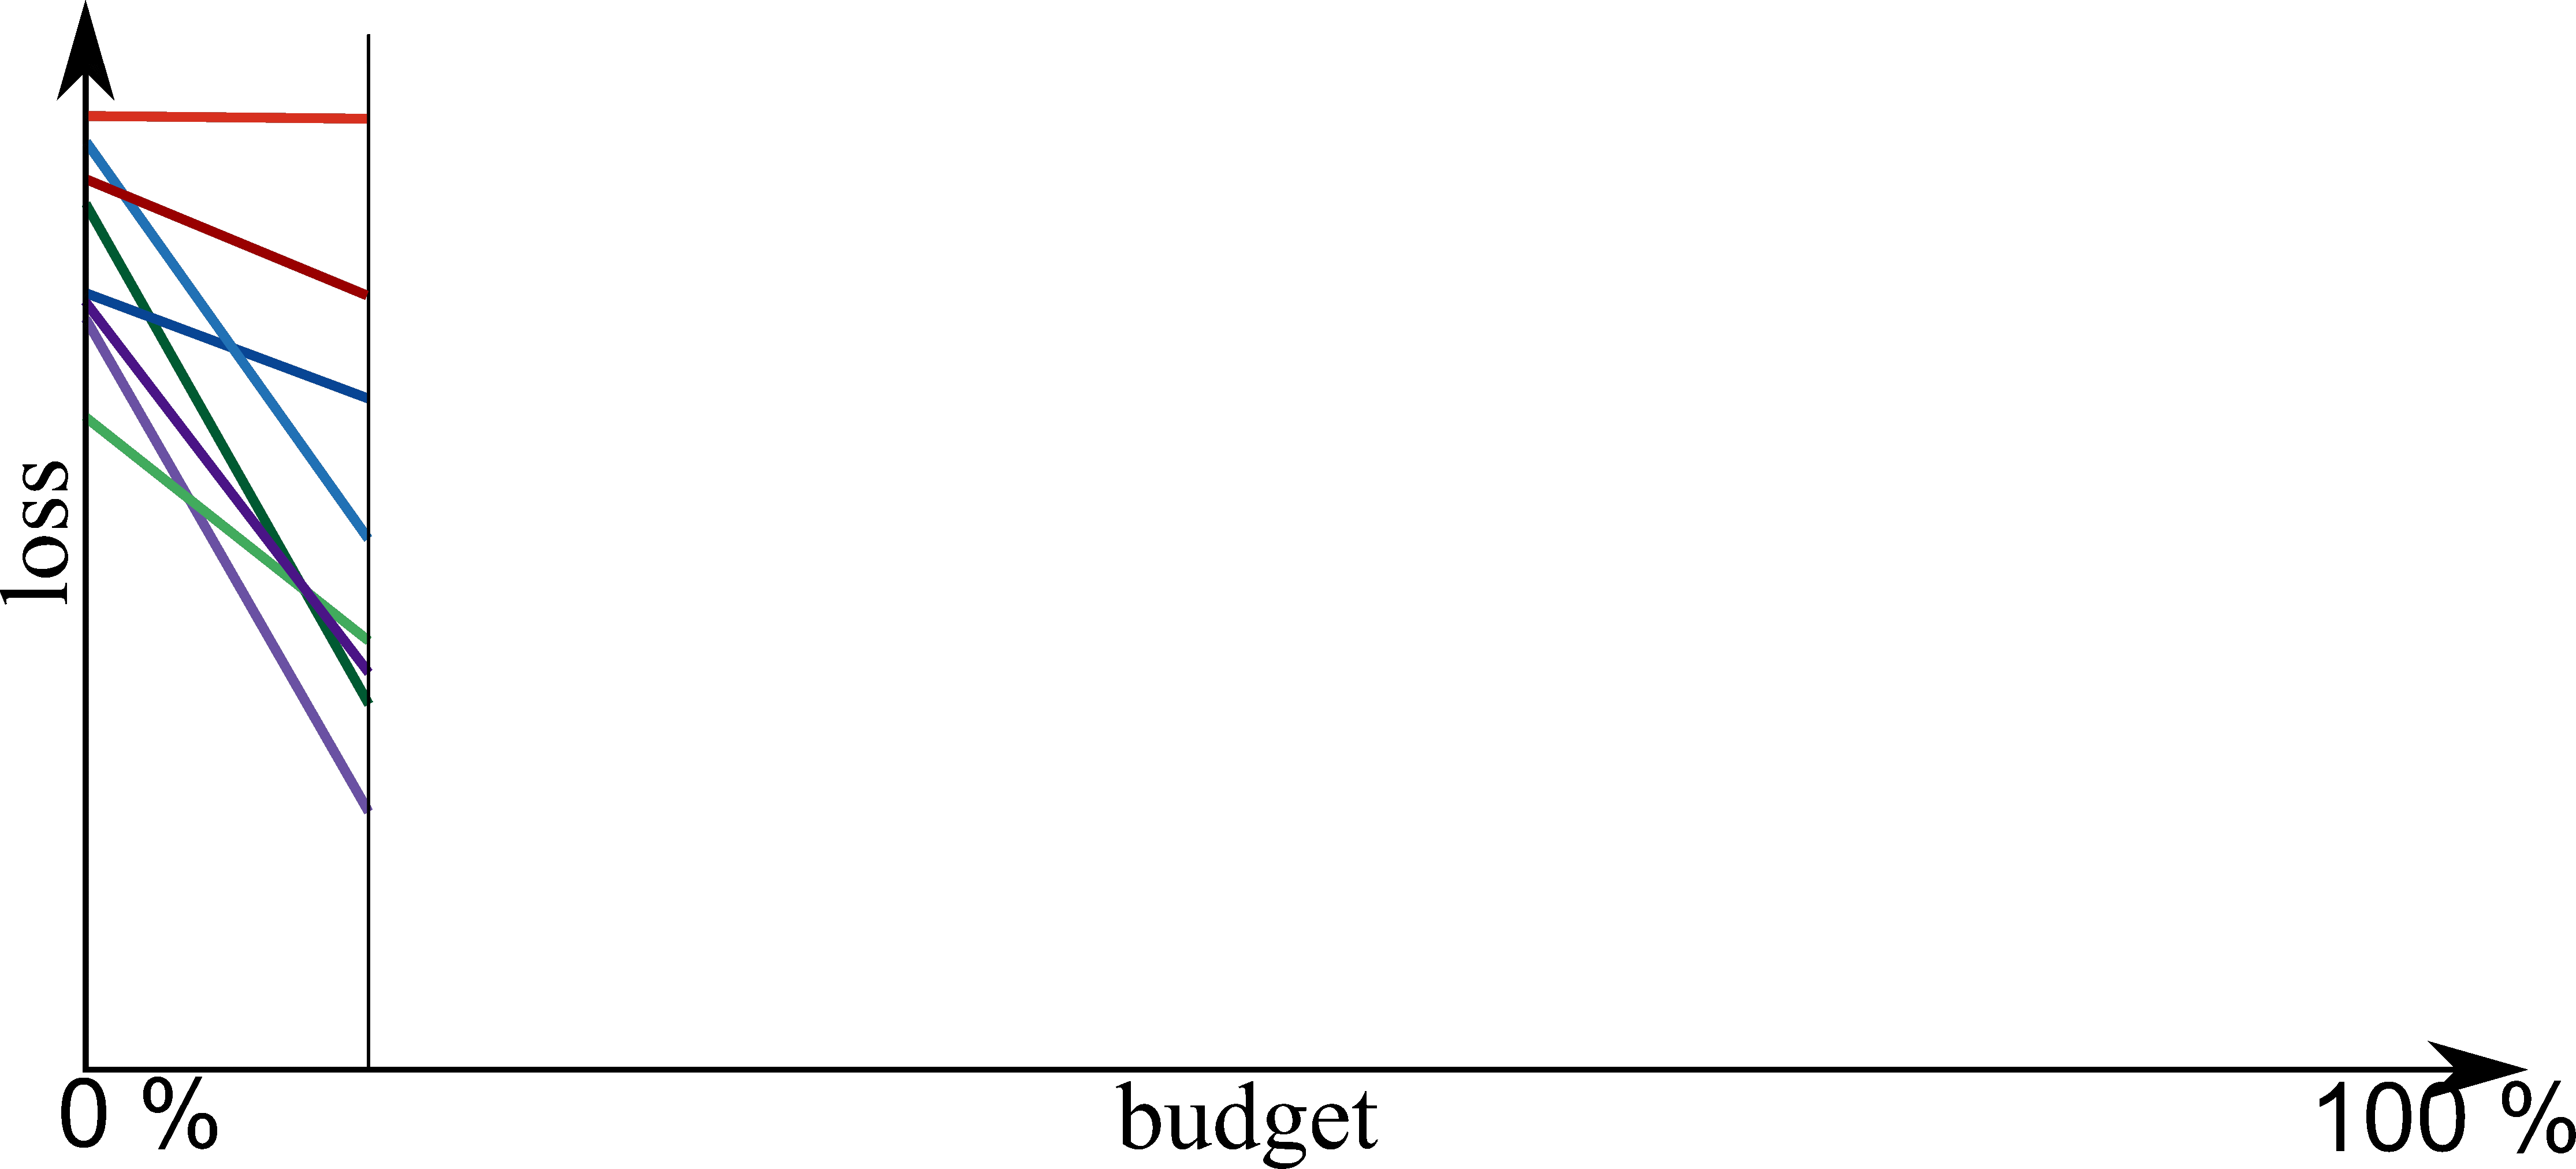
\includegraphics[width=\linewidth]{images/hyperband/SH-1.png}}
    \only<4>{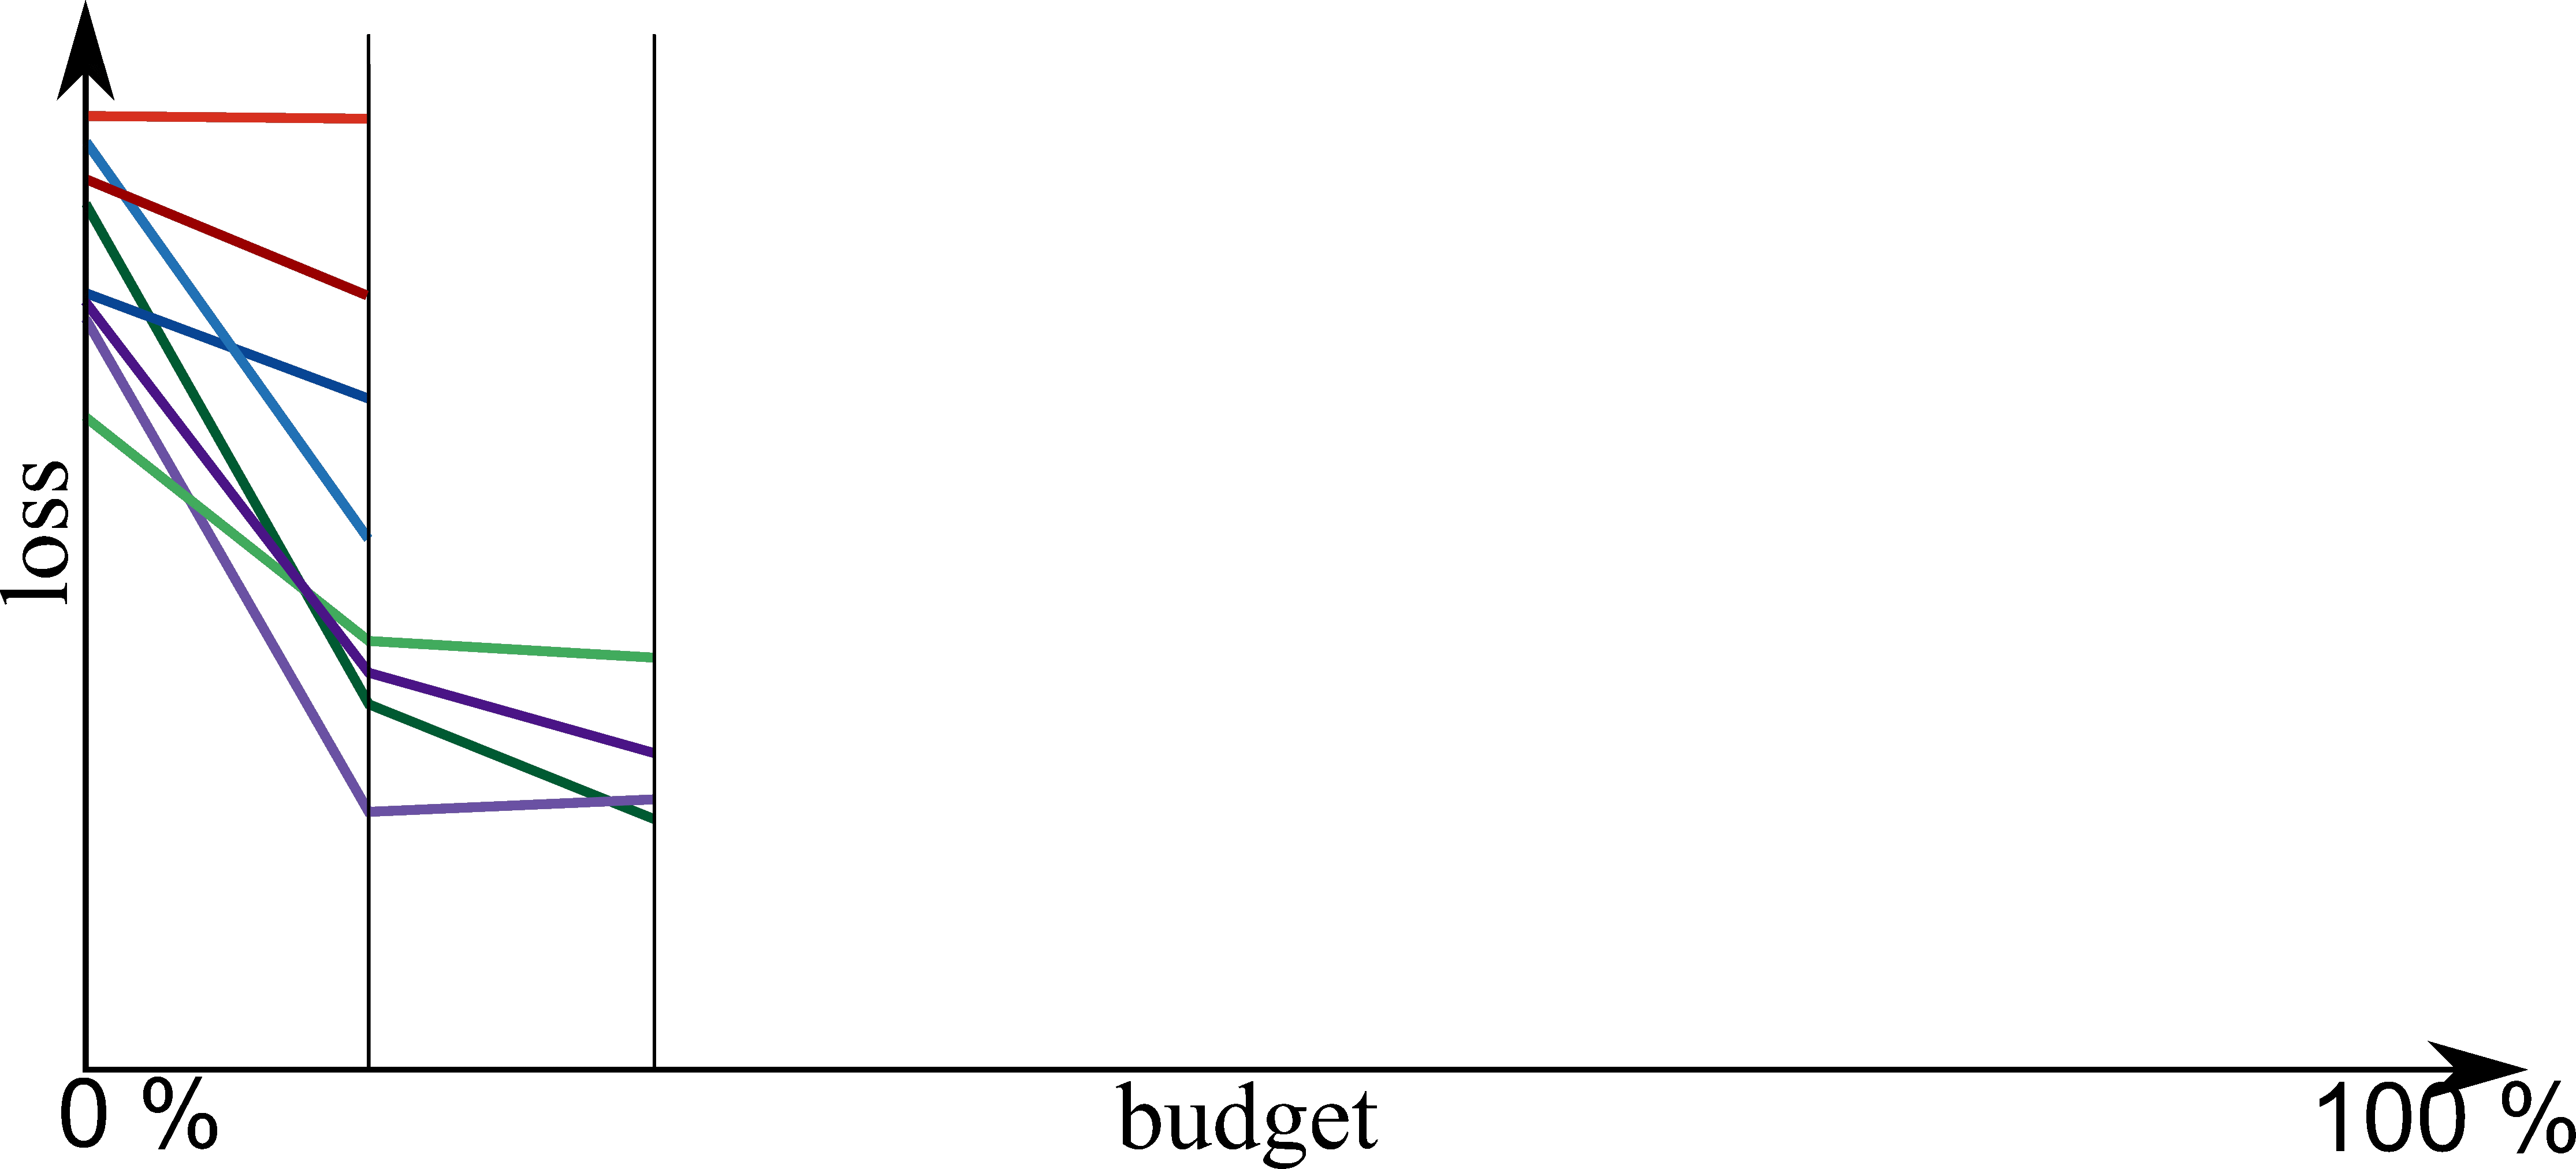
\includegraphics[width=\linewidth]{images/hyperband/SH-2.png}}
    \only<5>{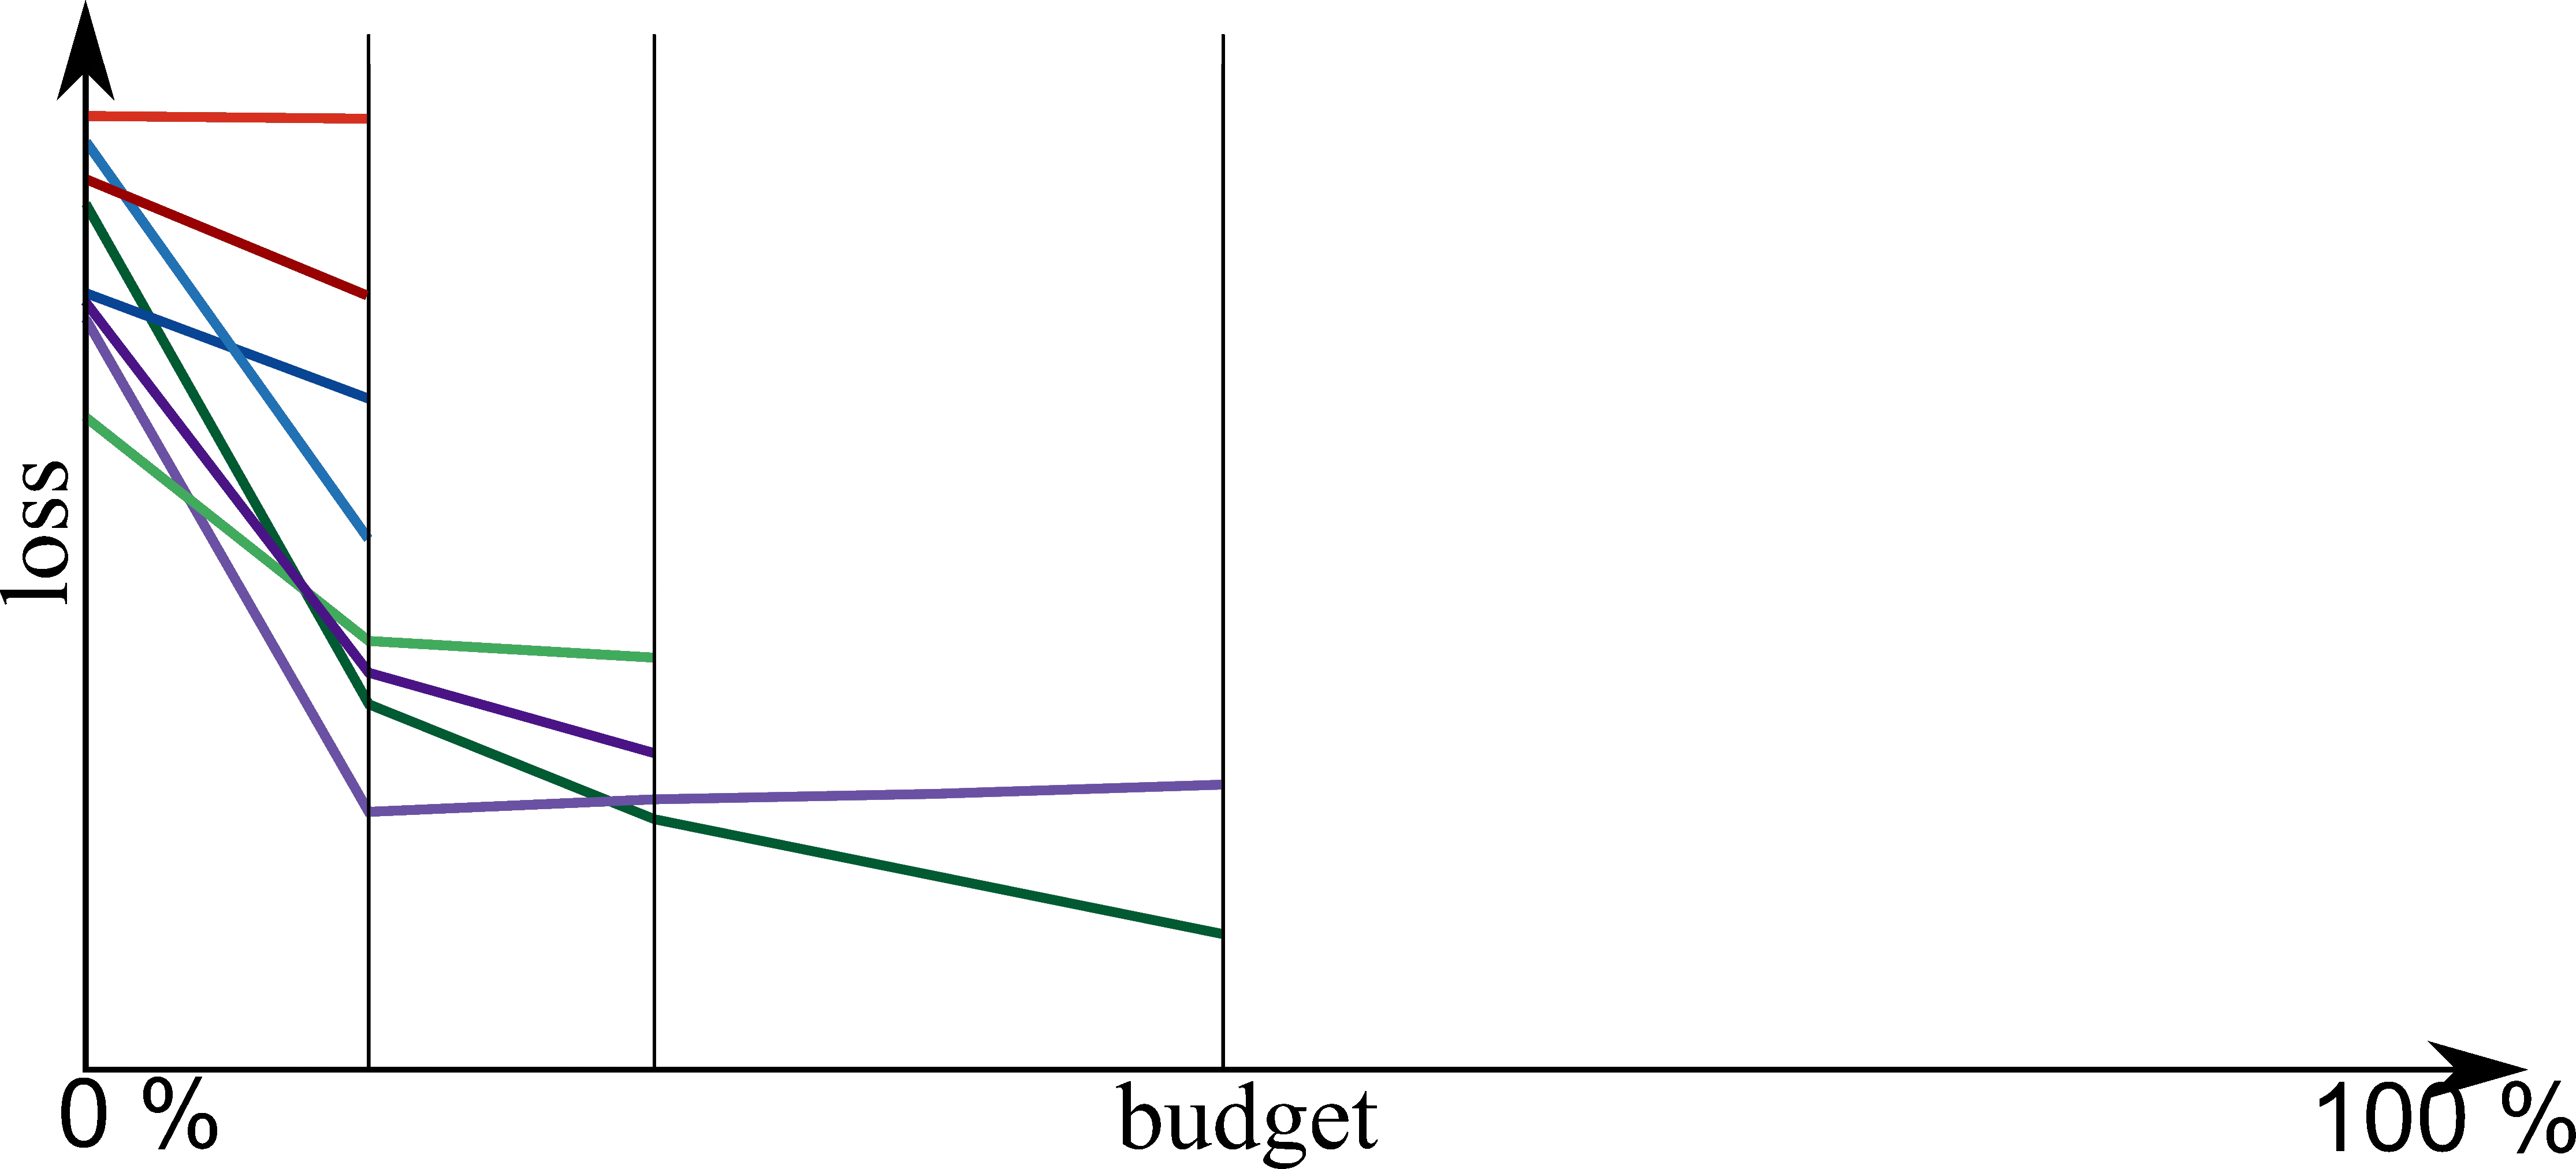
\includegraphics[width=\linewidth]{images/hyperband/SH-3.png}}
    \only<6>{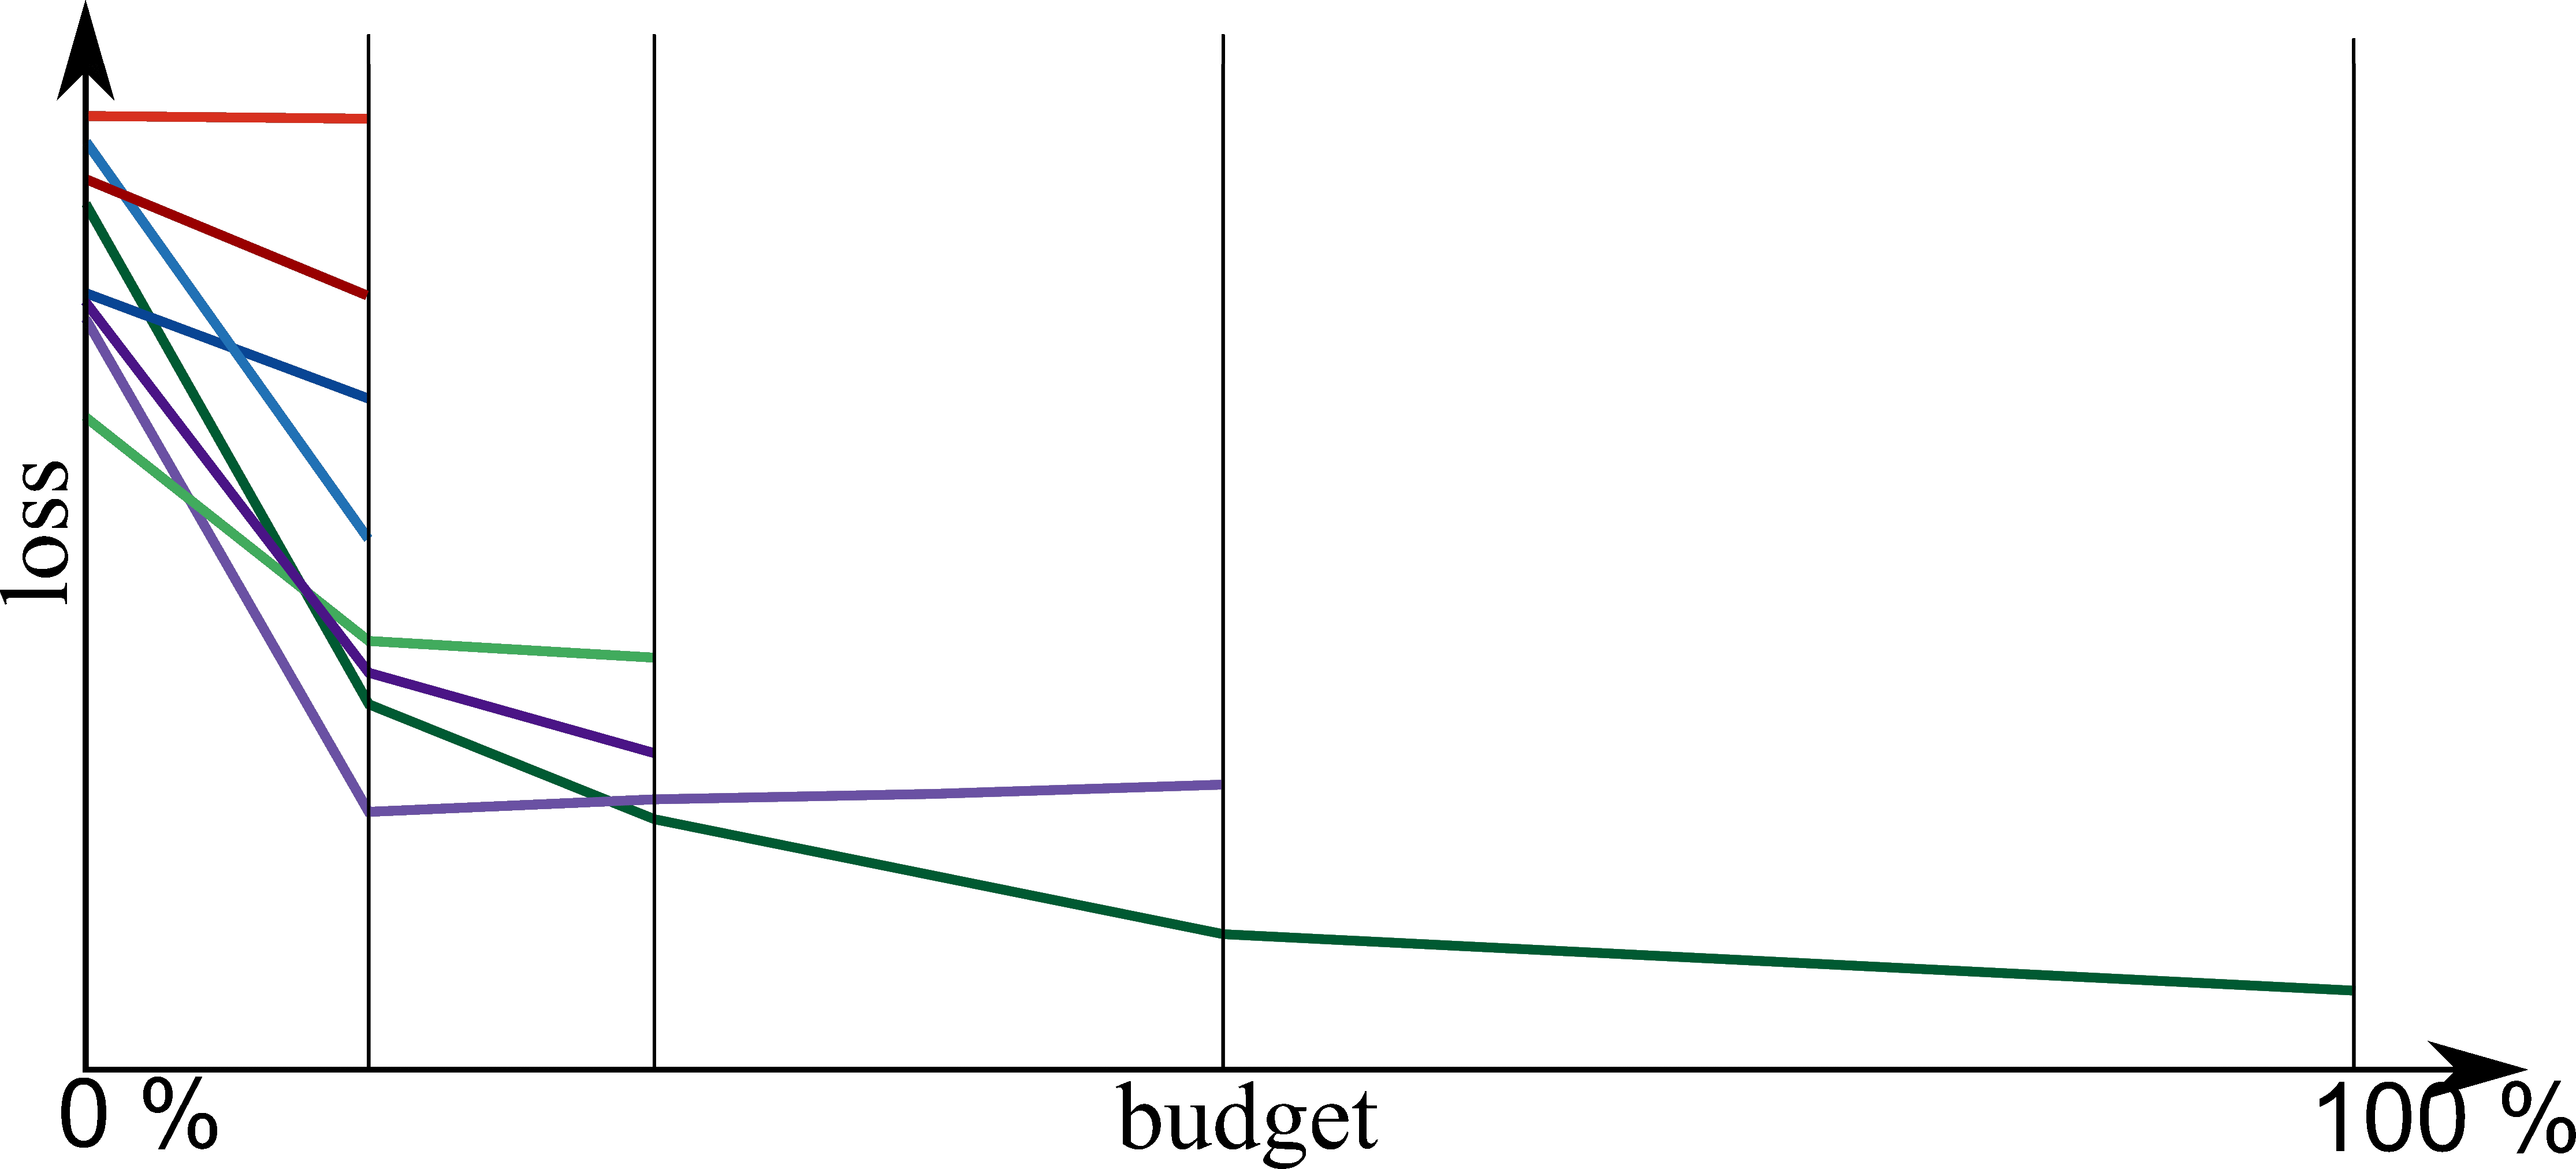
\includegraphics[width=\linewidth]{images/hyperband/SH-4.png}}

\end{figure}
\end{column}
\end{columns}
\vspace{-5em}
\begin{columns}
\begin{column}{.45\textwidth}
Given a budget $B$ and the number of configurations $n$ as an input:
\pause
\begin{itemize}
    \item Evaluate the performance of all configurations.
    \pause
    \item Drop the worst performing half.
    \pause
    \item Repeat until termination criterion is met e.g. maximum budget.

\end{itemize}
\end{column}

\begin{column}{.45\textwidth}
\end{column}

\end{columns}

\end{frame}

%-----------------------------------------------------------------------
%-----------------------------------------------------------------------

\begin{frame}{Successive Halving(SH): Algorithm}
\begin{algorithm}[H]
    %\DontPrintSemicolon
    \LinesNumbered
    \SetAlgoLined
    \setcounter{AlgoLine}{0}
    \SetKwInOut{Input}{Input}
    \DeclarePairedDelimiter\ceil{\lceil}{\rceil}
    \DeclarePairedDelimiter\floor{\lfloor}{\rfloor}
    \DeclarePairedDelimiter\abs{\lvert}{\rvert}
    
    \Input{ initial budget $b_0,$ maximum budget $b_{max},$ set of $n$ configurations $C=\{\conf_1, \conf_2,\dots, \conf_{n}\}$}
    $b=b_0$\\
    \While{$b\leq b_{max}$}{
    $L=\{\Tilde{\cost}(\conf,b):\conf \in C\}$;\
    
    $C=top_{k}(C,L,\lfloor\lvert C \rvert\ / \eta \rfloor)$;\
    
    $b=\eta \cdot b$;\
    }
    
 
        
    
    \caption{Pseudocode for SuccessiveHalving used by Hyperband as a subroutine}
\end{algorithm}

\end{frame}

%-----------------------------------------------------------------------

\begin{frame}{\emph{"n versus B/n" Problem}}
\begin{columns}

\begin{column}{.45\linewidth}
\begin{itemize}
    \item SH requires $B$ and $n$ as an input.
    \pause
    \item Given finite $B$, $B/n$ resources are allocated across the configurations.
    \pause
    \item Configurations need enough minimal resources to differentiate between them in terms of quality.
    \pause
\end{itemize}
\end{column}

\begin{column}{.45\linewidth}

\begin{figure}
    \centering
    \vspace{2em}
    \includegraphics[width=0.9\linewidth]{images/intro/differetiatingConfigurations.png}
    \pause
\end{figure}
\end{column}
\end{columns}

\vspace{-6.5em}
\begin{columns}

\begin{column}{.45\linewidth}
\begin{itemize}

    \item Issue: Optimal allocation strategy is unknown in practice.
    \pause
    \item Idea: Perform grid search over a feasible set of tuples of $n$ and minimal resource $r$. (Hyperband) 
\end{itemize}
\end{column}

\begin{column}{.45\linewidth}

\end{column}
    
\end{columns}
    
\end{frame}

%-----------------------------------------------------------------------
\begin{frame}{Hyperband}
\begin{itemize}
    \item Issue of successive halving (for a fixed B):
    \begin{itemize}
        \item Do you want to run many configurations with aggressive rejection?
        \item Or: Do you want to run few configurations with non-aggressive rejection?
    \end{itemize}
    \item Ideas:
    \begin{itemize}
        \item Add an outer loop to try different trade-offs between $\#$configurations and budget.
        \item Add further parameter: proportion of configurations discarded in each round of successive halving
    \end{itemize}
    \item Starts with many configurations that gets aggressively rejected.
    \item In later iterations, fewer configurations with more budget each.
    \item Returns: configuration with the smallest intermediate loss seen so far.
\end{itemize}
\end{frame}

%-----------------------------------------------------------------------

\begin{frame}{Hyperband: Algorithm}
\begin{minipage}{0.75\textwidth}
\begin{algorithm}[H]
    %\DontPrintSemicolon
    \LinesNumbered
    \SetAlgoLined
    \setcounter{AlgoLine}{0}
    \DeclarePairedDelimiter\ceil{\lceil}{\rceil}
    \DeclarePairedDelimiter\floor{\lfloor}{\rfloor}
    
    \Input{budgets $b_{min}$ and $b_{max}, \eta$}
    
    $s_{max}=\floor*{\log_{\eta}\frac{b_{max}}{b_{min}}}$;\
    
    \For{$s\in \{s_{max}, s_{max}-1, \dots, 0\}$}
    {
        sample $\eta=\lceil\frac{s_{max}+1}{s+1} \cdot\eta^{s}\rceil$;\
        
        run SH on them with $\eta^{s}\cdot b_{max}$;\
    }
 
        
    
    \caption{Pseudocode for Hyperband using SuccessiveHalving (SH) as a subroutine}
\end{algorithm}
\end{minipage}
\end{frame}
%-----------------------------------------------------------------------
%-----------------------------------------------------------------------
\begin{frame}{Tradeoffs between n and B/n}
\vspace{2em}
\begin{figure}
    \centering
    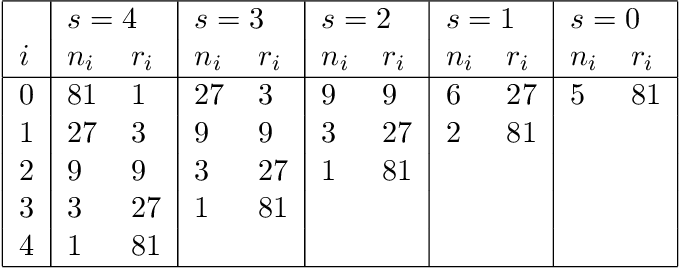
\includegraphics[width=0.7\textwidth]{images/hyperband/Hyperband_Table1-1.png}
    \caption{The values of $n_i$ and $r_i$ for the brackets of Hyperband corresponding to various values of $s$, when $R = 81$ and $\eta = 3$.}
\end{figure}

    
\end{frame}

%-----------------------------------------------------------------------
%-----------------------------------------------------------------------
\begin{frame}{Empirical comparison between individual brackets}
\begin{figure}
    \centering
    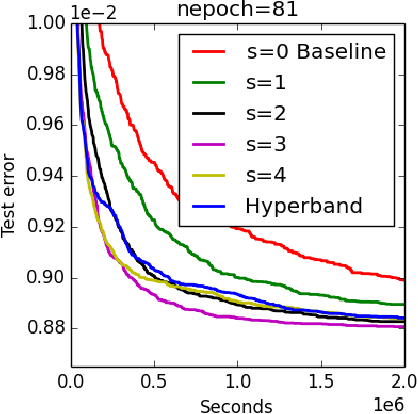
\includegraphics[width=0.4\textwidth]{w07_hpo_grey_box/images/hyperband/Hyperband_figure_3.png}
    \caption{Performance of individual brackets $s$ and Hyperband.}
\end{figure}
\begin{itemize}
    \item Hyperband is slower than SuccessiveHalving by a small factor if aggressive early-stopping is not suitable for the task.
\end{itemize}

    
\end{frame}

%-----------------------------------------------------------------------
\begin{frame}{Hyperband: Comparison}
\begin{figure}
    \centering
    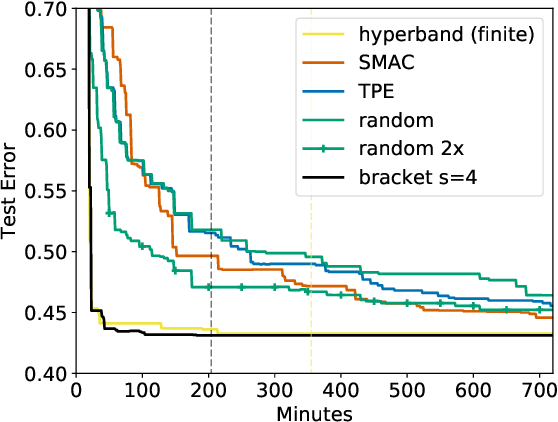
\includegraphics[width=0.55\textwidth]{w07_hpo_grey_box/images/hyperband/Figure_experiments.png}
    \caption{Average test error of the best kernel regularized least square classification model found by each searcher on CIFAR-10.}
\end{figure}

    
\end{frame}

%-----------------------------------------------------------------------

%-----------------------------------------------------------------------
\begin{frame}{Random Search vs. Hyperband}
\begin{itemize}
    \item In practice HB performs very well for small to medium budgets
    \item Outperforms random search and vanilla BO
    \item However, its convergence is limited by its reliance on randomly-drawn configurations
    \item With larger budgets its advantage over random search diminishes
\end{itemize}
\begin{figure}
    \centering
    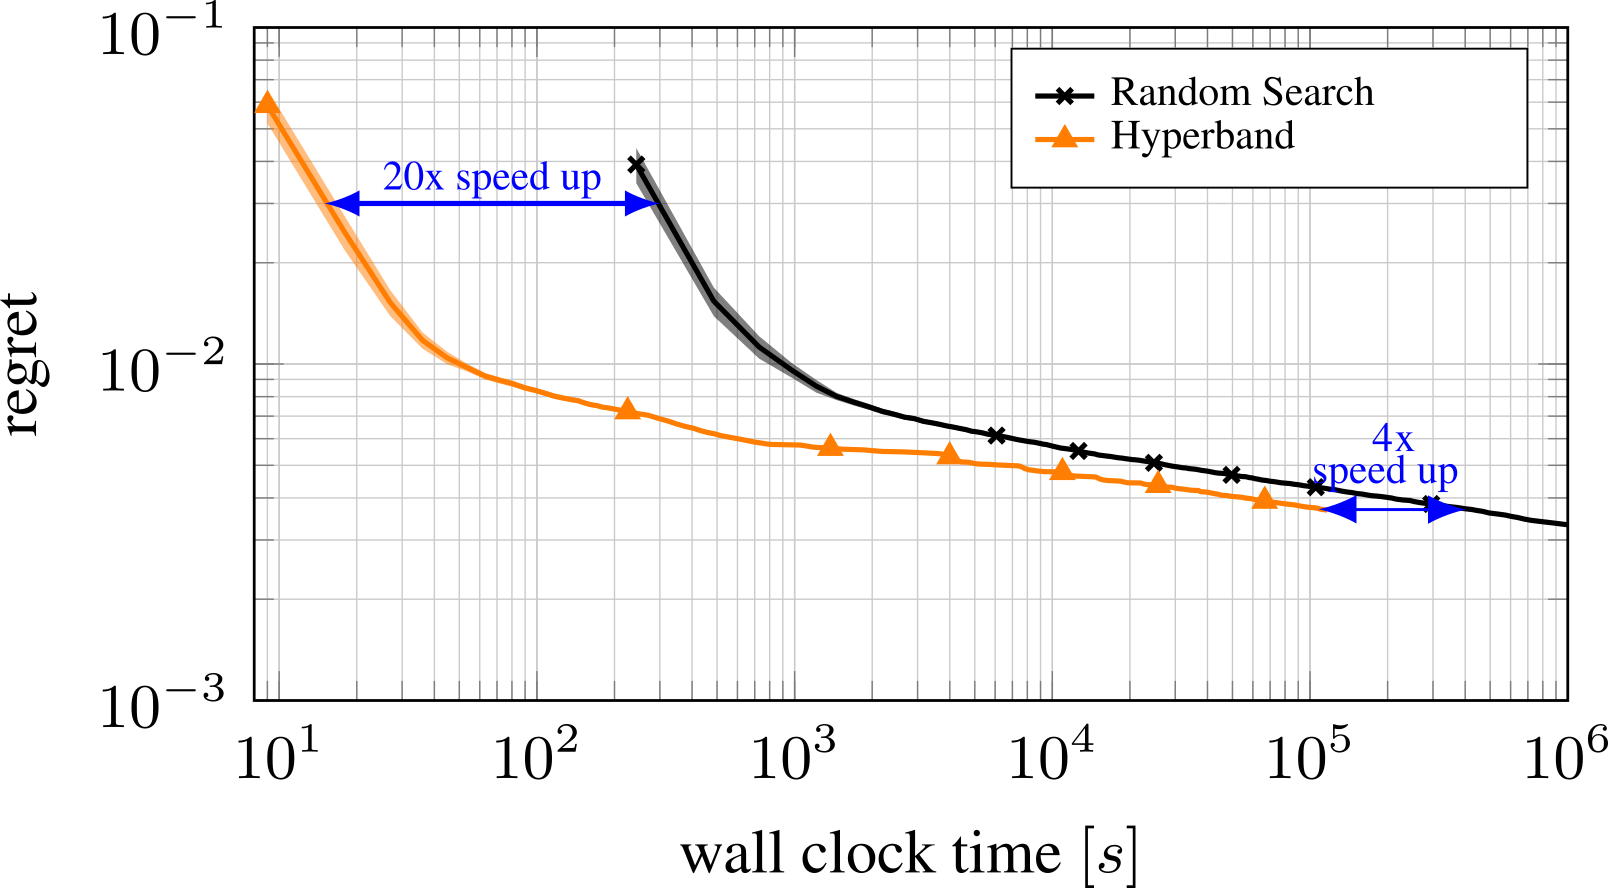
\includegraphics[width=0.6\textwidth]{images/hyperband/comparison_rs_hb.png}
\end{figure}


\end{frame}

%-----------------------------------------------------------------------

%----------------------------------------------------------------------
%----------------------------------------------------------------------
\begin{frame}[c]{}

TODO

\end{frame}
%-----------------------------------------------------------------------
%----------------------------------------------------------------------
\begin{frame}{BOHB: Algorithm}

\begin{algorithm}[H]
    %\DontPrintSemicolon
    \LinesNumbered
    \SetAlgoLined
    \setcounter{AlgoLine}{0}
    \DeclarePairedDelimiter\ceil{\lceil}{\rceil}
    \DeclarePairedDelimiter\floor{\lfloor}{\rfloor}
    \DeclarePairedDelimiter\abs{\lvert}{\rvert}
    
    \Input{observations D, fraction of random runs $\rho$, percentile $q$, number of samples $N_s$,
     minimum number of points $N_{min}$ to build a model, and bandwidth factor $b_w$}
    \Output{next configuration to evaluate}
    \lIf{$rand()<\rho$}{\Return{random configuration}}
    $b=\argmax \{D_b:\lvert D_b \rvert \geq N_{min}+2\}$
    
    \lIf{$b=\varnothing$}{\Return{random configuration}}
    
    fit KDEs according to Eqs. (2) and (3)
    
    Draw $N_s$ samples acoording to $l'(x)$
    
    \Return{sample with highest ratio $l(x)/g(x)$}
    
   
 
        
    
    \caption{Pseudocode for sampling in BOHB}
\end{algorithm}

\end{frame}
%-----------------------------------------------------------------------

%----------------------------------------------------------------------
%----------------------------------------------------------------------
\section{Success Stories}

\begin{frame}[c]{Large-scale meta-learning for hyperparameter optimization}

\begin{itemize}
    \item Facebook has an internal self-service machine learning system
    \item Non-ML departments can integrate highly optimized machine learning models into their workflow
    \item Hyperparameters of the ML models are optimized with Bayesian optimization
    \item Training data for the models changes over time \item Hyperparameters are constantly re-optimized using meta-learning Bayesian optimization as described in \lit{\href{https://arxiv.org/abs/1802.02219}{Feurer et al. 2018}}
    \begin{figure}
        \centering
        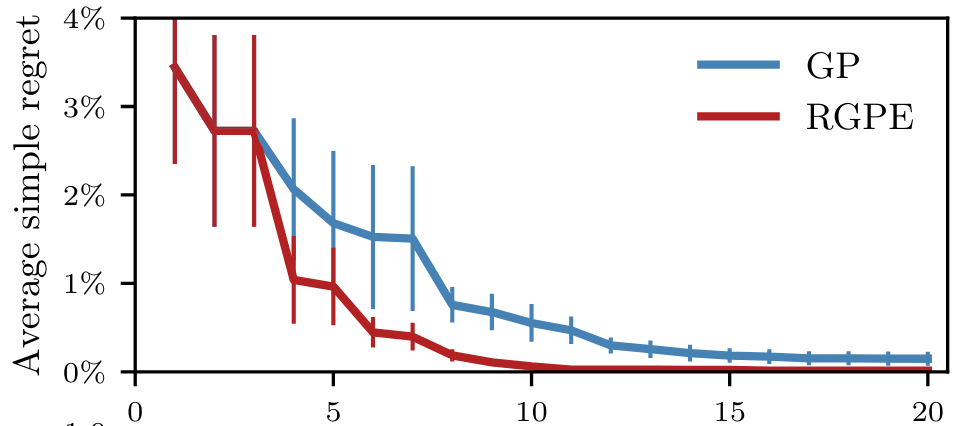
\includegraphics[width=0.5\textwidth]{images/success_stories/FB_RGPE.png}
        \caption{Bayesian optimization with meta-learning (RGPE) vs. vanilla Bayesian optimization (GP)}
    \end{figure}
\end{itemize}

\end{frame}

%-----------------------------------------------------------------------

\begin{frame}[c]{Auto-sklearn}
Extension of Auto-WEKA with focus on speed improvements and robustness:
\begin{figure}
    \centering
    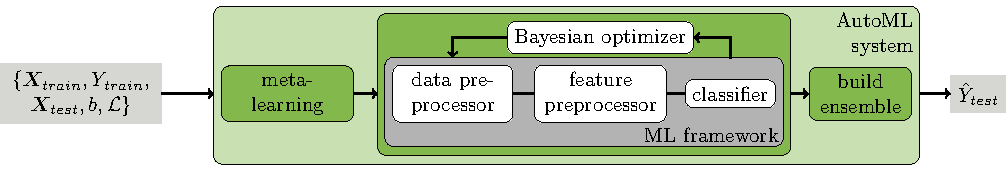
\includegraphics[width=0.9\textwidth]{images/success_stories/automlworkflow.pdf}
\end{figure}
\begin{itemize}
    \item Uses Meta-learning to warmstart Bayesian optimization
    \item Won the 1st AutoML challenge
    \item Open source (BSD) and trivial to use:
\end{itemize}
\begin{figure}
    \centering
    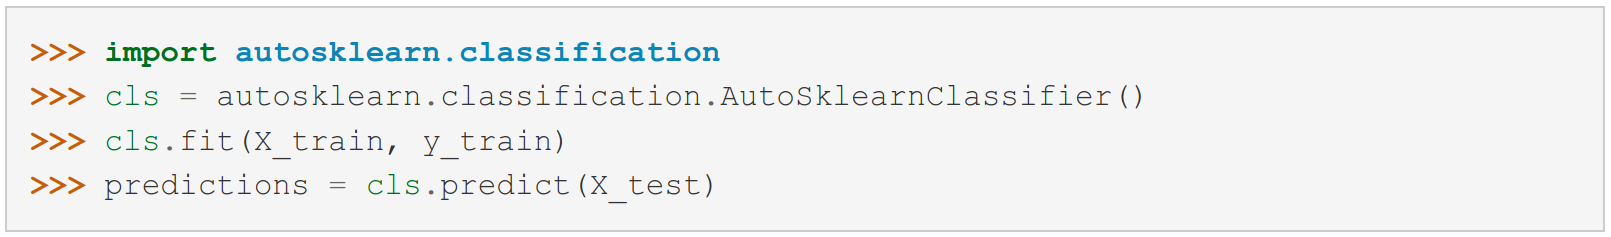
\includegraphics[width=0.9\textwidth]{images/success_stories/Auto-sklearn_01.png}
\end{figure}
Available at \href{automl.github.io/auto-sklearn}{automl.github.io/auto-sklearn}
\end{frame}

%-----------------------------------------------------------------------

\begin{frame}[c]{PoSH-Auto-sklearn}
Idea: integrate successive halving for further speed improvements:
\begin{itemize}
    \item Uses task-independent Meta-learning to warmstart Bayesian optimization
    \item Uses Successive Halving to quickly go through proposed configurations
    \item Won the 2nd AutoML challenge
\end{itemize}

\begin{figure}
    \centering
    \includegraphics[width=\textwidth]{images/success_stories/automl_bo_po_es.png}
\end{figure}

\hspace{12cm}\lit{\href{https://ml.informatik.uni-freiburg.de/papers/18-AUTOML-AutoChallenge.pdf}{Feurer et al. 2018}}
\end{frame}

%-----------------------------------------------------------------------




\end{document}
